\documentclass{article}

\usepackage[utf8]{inputenc}
\usepackage[french]{babel}

\usepackage{lmodern}
\usepackage{graphicx}
\usepackage{hyperref}
\usepackage{graphicx}
\usepackage{natbib}
\usepackage{tcolorbox}
\usepackage{xcolor}
\usepackage{geometry}
\graphicspath{ {./res/} }

\definecolor{needcolor}{HTML}{007ACC}
\definecolor{nonfunctionnalneedcolor}{HTML}{9722ff}
\definecolor{subneedcolor}{HTML}{28A745}

\tcbuselibrary{skins, breakable}
\newtcolorbox{needbox}[1][]{
  colframe=needcolor,
  colback=needcolor!10,
  coltitle=white,
  fonttitle=\bfseries,
  title=#1,
  breakable,
  enhanced,
  sharp corners=all
}

\newtcolorbox{nonfunctionnalneedbox}[1][]{
  colframe=nonfunctionnalneedcolor,
  colback=nonfunctionnalneedcolor!10,
  coltitle=white,
  fonttitle=\bfseries,
  title=#1,
  breakable,
  enhanced,
  sharp corners=all
}

\newtcolorbox{subneedbox}[1][]{
  colframe=subneedcolor,
  colback=subneedcolor!10,
  coltitle=white,
  fonttitle=\bfseries,
  title=#1,
  breakable,
  enhanced,
  sharp corners=all
}


\author{
    Valentin Jonquière,
    Mathilde Chollon,
    Denis Demirci,
    Iwen Jomaa,
    Jonathan Landry
}

\title{Rapport Préliminaire projet de programmation, Échecs en Java}

\begin{document}

\maketitle

\pagebreak

\tableofcontents

\pagebreak

\section{Contexte du sujet}
\subsection{Sujet choisi}
Nous avons choisi le sujet '\textit{les échecs}' car nous avons abordé ce jeu
plusieurs fois et dans différentes disciplines. Nous avions par exemple illustré un 
cours d'intelligence artificielle au semestre dernier avec celui-ci, mais 
également un cours d'algorithmie par le passé. Nous avons donc quelques connaissances 
utiles pour réaliser certains des besoins et qui nous permettent plus généralement de ne pas
découvrir entièrement le sujet.

\subsection{Existant}
Les échecs étant un jeu universel, ils ont été étudiés et un grand nombre de papiers scientifiques
sont disponibles. Ceux-ci nous seront très utiles tout au long du projet, car ils concernent des
besoins différents. Tout d'abord une grande partie des papiers que nous allons utiliser sont en rapport
avec la partie intelligence artificielle du développement. C'est pour cela que nous avons par exemple
choisi de nous baser sur l'article `Programming a computer for playing chess' \cite{Shannon1950}, 
puisqu'il possède une partie consacrée à la construction d'heuristiques efficace pour les échecs.
Nous avons également basé nos recherches sur la thèse `Using Monte Carlo Tree Search to play chess' \cite{Kral2021}
de Jakub Král sur l'utlisation de différents algorithmes au service des échecs, tels que AlphaBeta ou
Monte Carlo Tree Seach. Pour la partie intelligence artificielle, nous avons choisi de nous baser sur le 
`Zobrist hashing' \cite{ZobristHashing} afin de ne pas réévaluer des positions déjà évaluées lors de la 
recherche du meilleur coup à jouer par le joueur artificiel \ref{Zobrist}. Nous avons également orienté
nos recherches sur la représentation du jeu d'échecs par les bitmaps (plateau, représentation des coups) \cite{Bijl2021}.
Pour finir, nous avons utilisé un papier plus général, mais contenant des informations sur le développement
d'un moteur d'échecs en java \cite{PaulDailly}. Nous nous servons également des deux articles présents sur 
notre repository Gitlab, \cite{Bitboards} et \cite{GameBitboards}, qui concernent aussi les Bitboards.

\subsection{Langage de programmation choisi}
Avec ce sujet, nous avions 3 choix de langage possibles :
\begin{itemize}
    \item Le langage C
    \item Le Java
    \item Le Python
\end{itemize}
Même si nous avons dû faire un choix rapidement, nous avons d'abord développé les
avantages et inconvenants de chacun de ces langages. De plus, nous nous étions mis
d'accord sur quelques besoins essentiels auquel certains des langages ci-dessus 
n'aurait pas (ou difficilement) pu répondre.
Tout d'abord nous souhaitions pouvoir développer notre logiciel sous forme de modules
complémentaires, pour plusieurs raisons.
\begin{itemize}
    \item Nous avons convenu de baser les 8 semaines de code en se concentrant sur 
    des blocs de 2 semaines avec, pour chaque bloc, une liste de 2 ou 3 modules à développer.
    \item Isoler les bugs dans chaque module afin d'avoir moins de problèmes lors de la fusion
    des modules.
    \item Facilité de maintien. Avec 8 semaines de code, il est essentiel que nous possédions
    un logiciel organisé afin de ne pas avoir à `fouiller' dans le code écrit la première semaine
    lors de la finalisation du projet.
    \item Utilisation de la programmation objet. Même s'il n'y a pas d'extension de prévue,
    ce paradigme est le plus simple et adopté lors du développement d'un jeu.
\end{itemize}

\subsubsection{Langage C}
La première option qui nous était proposée été le langage C. Le projet contenant des besoins posant
des contraintes de performances (cf. besoin), ce langage a donc semblé être une bonne idée, car il est
de loin celui permettant d'obtenir un logiciel performant. Cependant, celui-ci ne proposant pas de 
possibilité de développement objet, nous aurions dû faire une grosse concession dès le choix du langage.
De plus, la gestion de la mémoire étant à la charge du développeur, nous aurions pu rester bloqué un temps
précieux sur un pointeur mal alloué. Cette gestion de la mémoire apporte également le problème des fuites
mémoire qui demandent, elle aussi, parfois beaucoup de travail pour être résolues.

\subsubsection{Python}
Nous pouvions également utiliser \textit{Python} pour réaliser ce projet. Cependant, le fait que ce langage
soit non typé a vite écarté ce choix. En effet, les types étant vérifiés directement à l'exécution, il est
beaucoup plus dangereux d'avoir une ligne non couverte par un test (il faut donc un coverage maximal). Il y
a donc le danger de laisser des erreurs de typages qui ne sont découverte uniquement lorsqu'une partie du code
est exécutée après la livraison du code.

\subsubsection{Java}
Nous avons donc fini par opter pour \textit{Java}. En effet, il permet tout comme \textit{Python} de faire
de la programmation objet, mais avec plus de rigueur. Étant conçu pour le développement objet, il y a moins
de chance de mélanger plusieurs paradigmes et de se retrouver avec un code mi-objet/mi-impératif. De plus,
le typage statique permet d'avoir une meilleure stabilité grâce à la détection des erreurs de types à la 
compilation et permet également d'avoir un code plus prévisible. Enfin, les plus projets réalisés en licence
et en master étant souvent des projets java, tous les membres du groupe connaissent ce langage ainsi que ses
outils et environnements de développement. Cela permettra de gagner du temps lors de la mise en place du projet. 

\section{Explication du sujet}
\subsection{Règles du jeu}
Le jeu d'échecs contient beaucoup de règles parfois techniques, mais dont l'objectif reste simple à comprendre :
 il faut mettre le roi adverse en \textbf{échec et mat} pour gagner la partie. Cela signifie que le roi est attaqué 
 mais n'a aucun coup légal pour se défendre de cette attaque.

\subsubsection{L'échiquier et les pièces}
Les échecs se jouent sur un échiquier de 64 cases disposé en 8x8. Chaque joueur commence la partie avec 16 pièces :
\begin{itemize}
    \item 1 roi
    \item 1 dame
    \item 2 tours
    \item 2 cavaliers
    \item 2 fous
    \item 8 pions
\end{itemize}

\begin{minipage}{\textwidth}
    \centering
    Voici l'échiquier au début de la partie. \\
    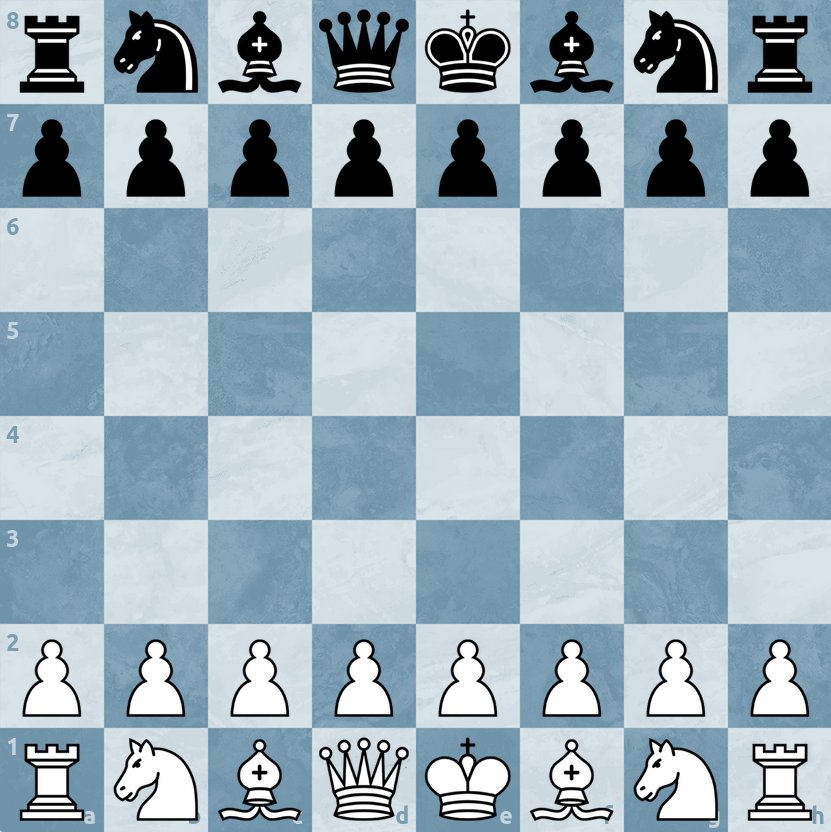
\includegraphics[width=0.6\textwidth]{jeuDepart.png}
    \vspace{0.5cm}
\end{minipage}

Le joueur avec les pièces blanches commence. Ensuite, chaque joueur joue à tour de rôle, un déplacement de pièce par tour.

\subsubsection{Déplacements des Pièces}
Les déplacements sont propres à chaque type de pièce :
\vspace{0.5cm}

\begin{itemize}
    \item \begin{minipage}{0.45\textwidth}
        \textbf{Déplacement du pion :} \\
        Le pion avance uniquement en ligne droite, d'une case à la fois. Toutefois, lors de son premier déplacement, 
        il a la possibilité d'avancer de deux cases. Contrairement à son déplacement habituel, le pion capture les pièces
         adverses en diagonale, en se déplaçant d'une case.
    \end{minipage}
    \hspace{0.05\textwidth}
    \begin{minipage}{0.45\textwidth}
        \centering
        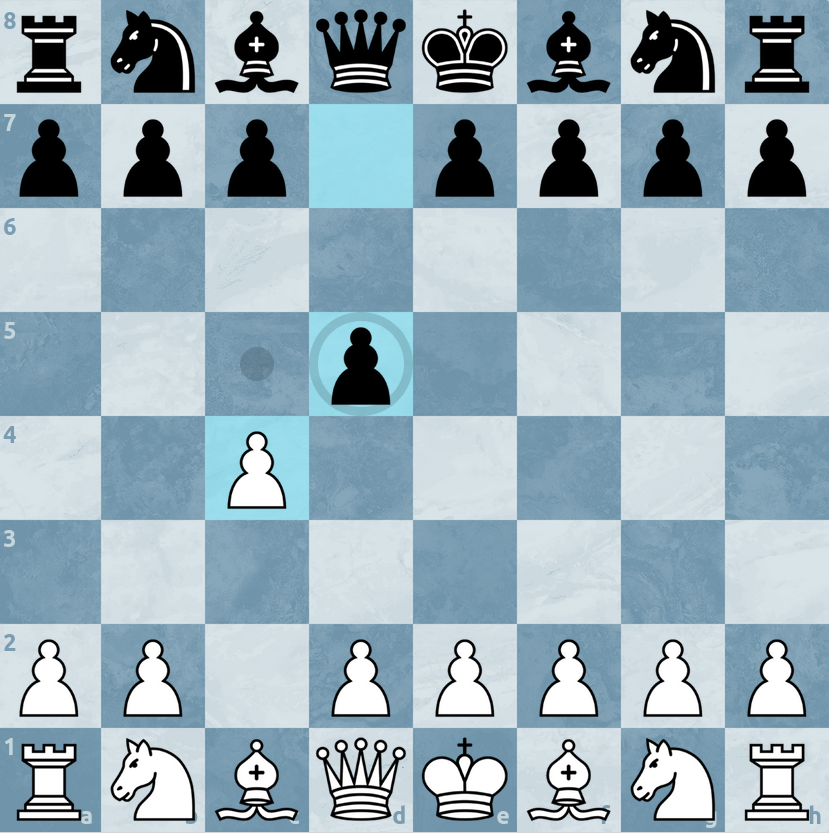
\includegraphics[width=\textwidth]{pionMove.png}
    \end{minipage}

    \vspace{0.5cm}

    \item \begin{minipage}{0.45\textwidth}
        \textbf{Déplacement du cavalier :} \\
        Le cavalier a un déplacement unique en forme de "L", ce qui signifie qu'il se déplace de deux cases dans une direction,
        puis d'une case perpendiculairement (ou inversement). C'est la seule pièce capable de sauter par-dessus d'autres 
        pièces sur l'échiquier.
    \end{minipage}
    \hspace{0.05\textwidth}
    \begin{minipage}{0.45\textwidth}
        \centering
        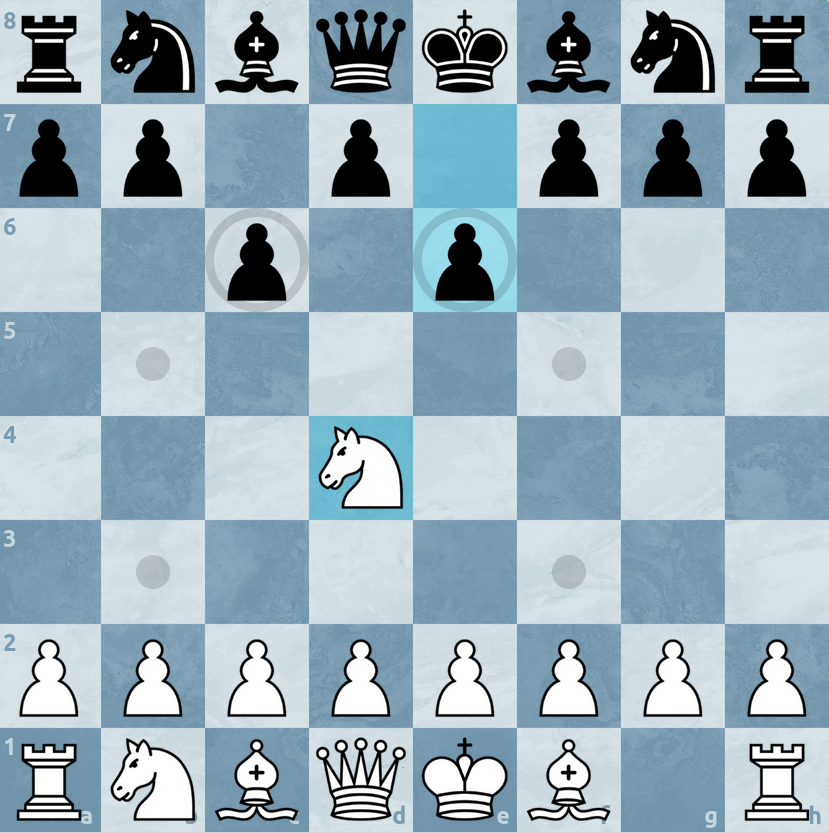
\includegraphics[width=\textwidth]{cavalierMove.png}
    \end{minipage}

    \vspace{0.5cm}

    \item \begin{minipage}{0.45\textwidth}
        \textbf{Déplacement du fou :} \\
        Le fou se déplace en diagonale sur un nombre illimité de cases, tant qu'il n'est pas bloqué par une autre pièce.
         Chaque fou reste toujours sur des cases de la couleur d'où il a commencé (blanches ou noires).
    \end{minipage}
    \hspace{0.05\textwidth}
    \begin{minipage}{0.45\textwidth}
        \centering
        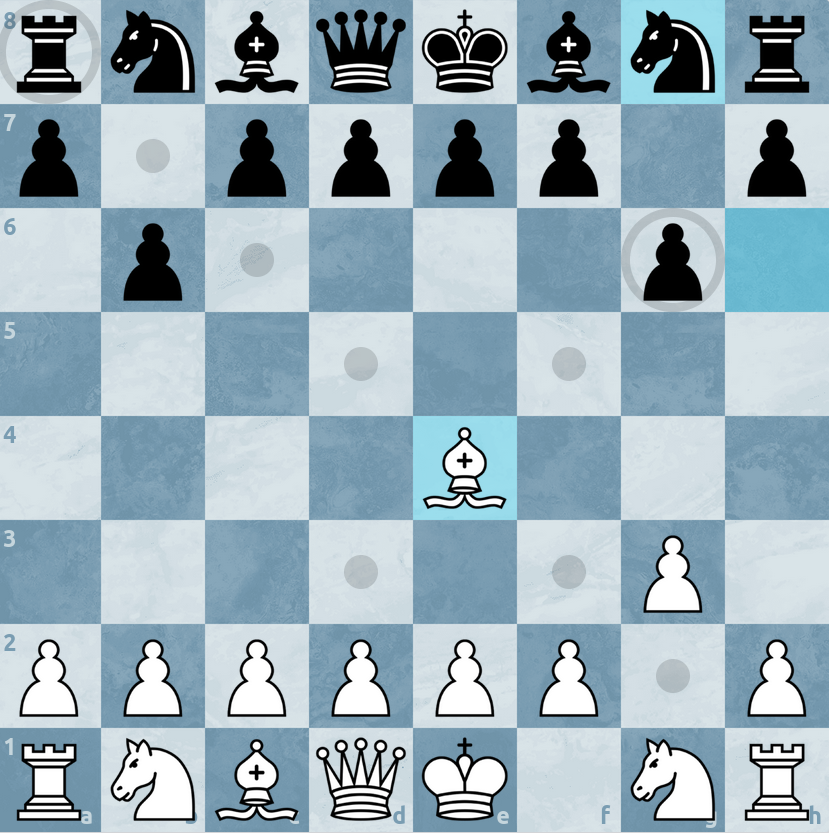
\includegraphics[width=\textwidth]{fouMove.png}
    \end{minipage}

    \vspace{0.5cm}

    \item \begin{minipage}{0.45\textwidth}
        \textbf{Déplacement de la tour :} \\
        La tour peut se déplacer de manière illimitée en ligne droite, que ce soit horizontalement ou verticalement.
        Sa puissance réside dans sa capacité à contrôler des colonnes et des rangées entières.
    \end{minipage}
    \hspace{0.05\textwidth}
    \begin{minipage}{0.45\textwidth}
        \centering
        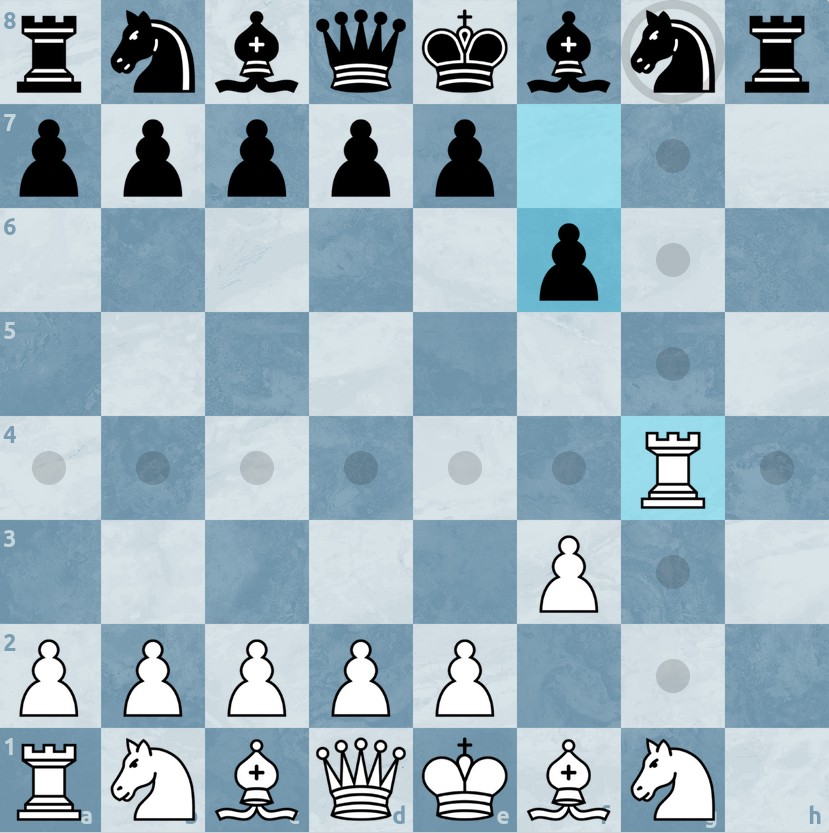
\includegraphics[width=\textwidth]{tourMove.png}
    \end{minipage}

    \vspace{0.5cm}

    \item \begin{minipage}{0.45\textwidth}
        \textbf{Déplacement de la dame :} \\
        La dame est la pièce la plus puissante du jeu. Elle combine les capacités de déplacement du fou et de la tour:
        elle peut se déplacer d'un nombre illimité de cases horizontalement, verticalement ou en diagonale.
    \end{minipage}
    \hspace{0.05\textwidth}
    \begin{minipage}{0.45\textwidth}
        \centering
        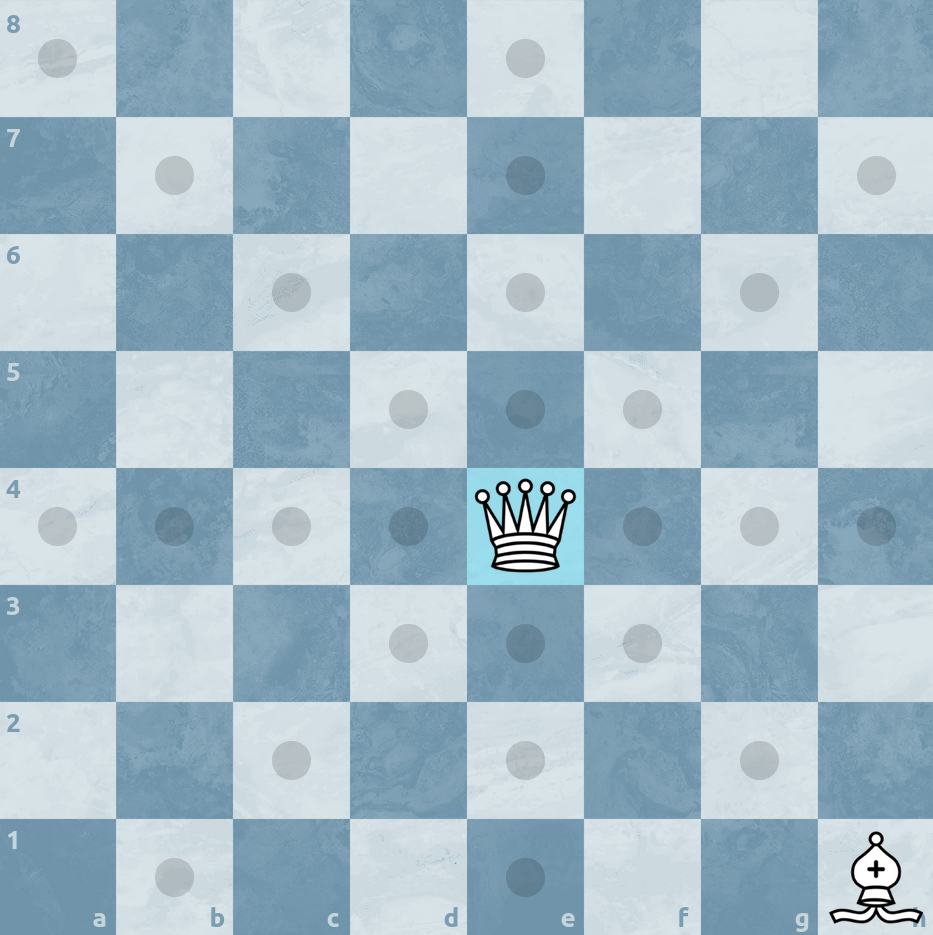
\includegraphics[width=\textwidth]{dameMove.png}
    \end{minipage}

    \vspace{0.5cm}

    \item \begin{minipage}{0.45\textwidth}
        \textbf{Déplacement du roi :} \\
        Le roi peut se déplacer d'une case dans n'importe quelle direction: horizontalement, verticalement ou en diagonale.
        Bien qu'il soit la pièce la plus importante, son mouvement limité le rend vulnérable.
    \end{minipage}
    \hspace{0.05\textwidth}
    \begin{minipage}{0.45\textwidth}
        \centering
        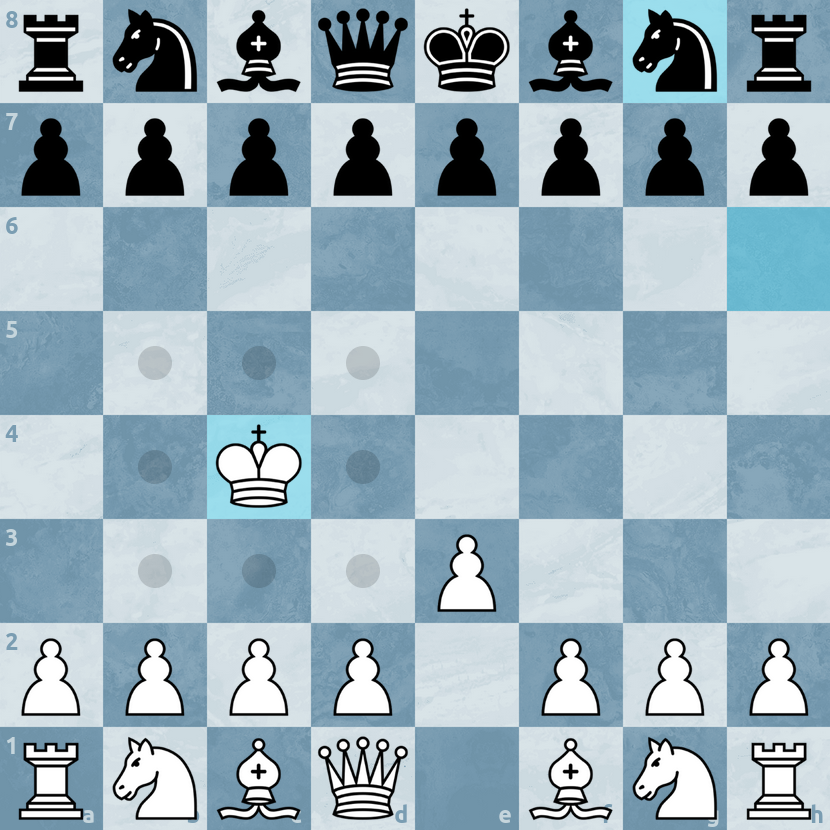
\includegraphics[width=\textwidth]{roiMove.png}
    \end{minipage}

\end{itemize}

\vspace{0.5cm}

Parfois, les déplacements peuvent être limités par des règles spécifiques comme le \textbf{clouage}. Voyons ces règles en détail.

\subsubsection{Règles Spécifiques}
\paragraph{-Clouage} Si une pièce défend une attaque au roi en se positionnant devant cette dernière, on dit qu'elle est \textbf{clouée}
 et ne peut pas bouger. En effet, il est interdit de mettre son roi en échec volontairement par l'une de ses propres actions.

 \noindent
 \begin{minipage}{0.48\textwidth}
     \centering
     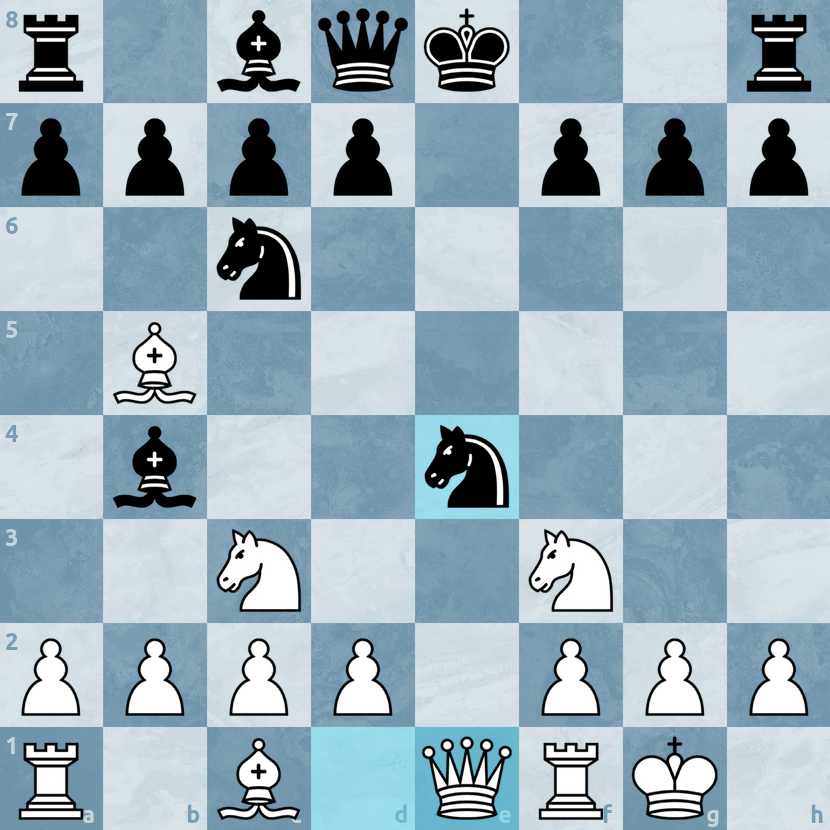
\includegraphics[width=\textwidth, height=\textwidth]{clouage1.png}
     \vspace{0.5cm}
    \textbf{Exemple de clouage}
 \end{minipage}
 \hfill
 \begin{minipage}{0.48\textwidth}
     \centering
     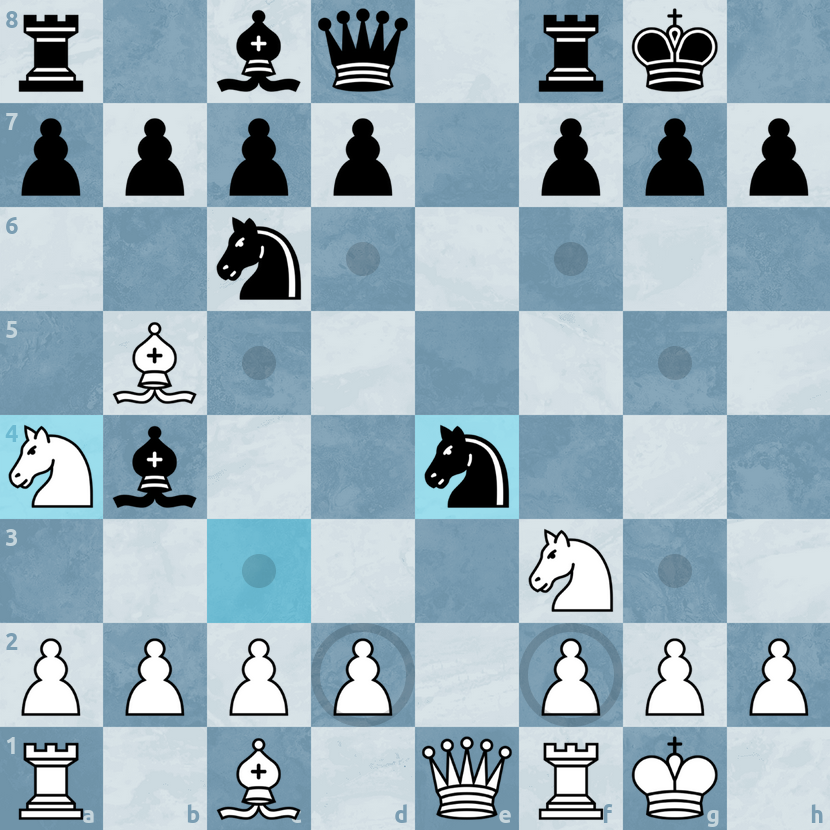
\includegraphics[width=\textwidth, height=\textwidth]{clouage2.png}
     \vspace{0.5cm}
 \end{minipage}

\paragraph{-Roc} Le \textbf{roc} est un mouvement spécial impliquant le roi et une des tours, sous certaines conditions :
\begin{itemize}
    \item Le roi et la tour concernés n'ont jamais bougé depuis le début de la partie.
    \item Le roi ne doit pas être en échec, et aucune des cases qu'il traverse ou sur laquelle il atterrit ne doit être attaquée.
    \item Il ne doit y avoir aucune pièce entre le roi et la tour.
\end{itemize}

\noindent
\begin{minipage}{0.48\textwidth}
    \centering
    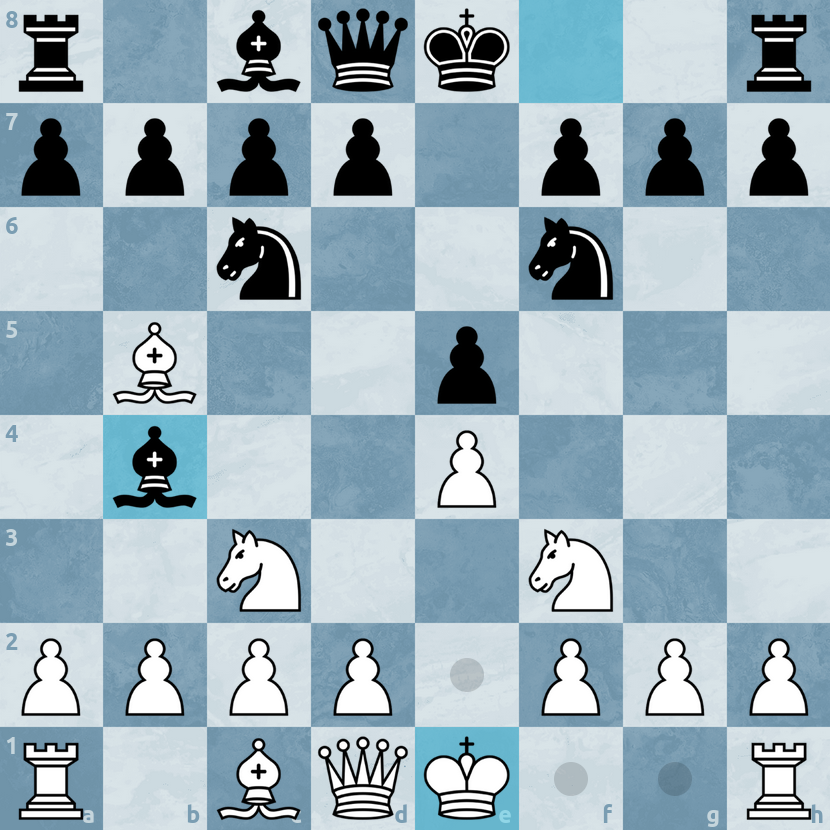
\includegraphics[width=\textwidth, height=\textwidth]{roc1.png}
    \vspace{0.5cm}
   \textbf{Exemple de roc}
\end{minipage}
\hfill
\begin{minipage}{0.48\textwidth}
    \centering
    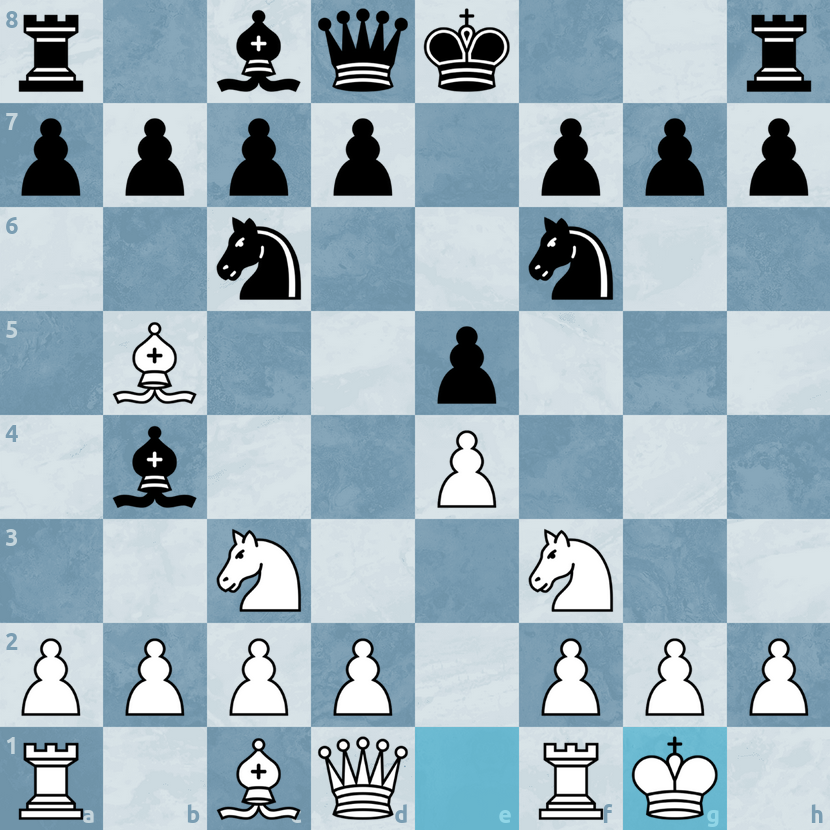
\includegraphics[width=\textwidth, height=\textwidth]{roc2.png}
    \vspace{0.5cm}
\end{minipage}

\paragraph{-Prise en Passant} Si un pion adverse avance de deux cases depuis sa position initiale et finit à côté d'un de nos pions,
 on peut le capturer \textbf{en passant}, mais uniquement au coup suivant.

 \noindent
 \begin{minipage}{0.48\textwidth}
     \centering
     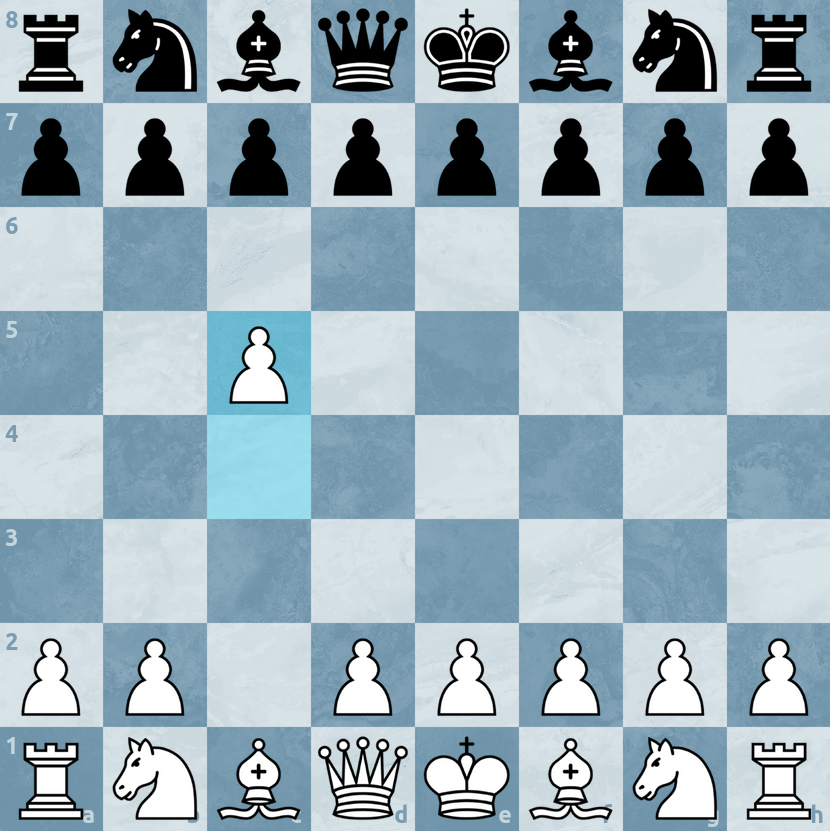
\includegraphics[width=\textwidth, height=\textwidth]{enpassant1.png}
     \vspace{0.5cm}
    \textbf{Exemple de en passant}
 \end{minipage}
 \hfill
 \begin{minipage}{0.48\textwidth}
     \centering
     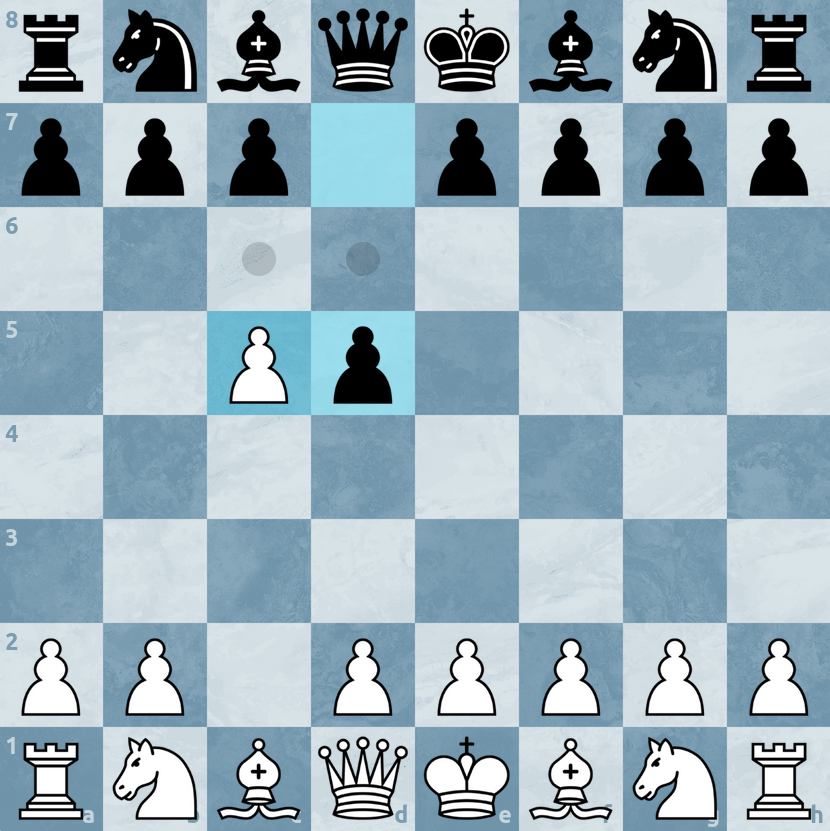
\includegraphics[width=\textwidth, height=\textwidth]{enpassant2.png}
     \vspace{0.5cm}
 \end{minipage}

\paragraph{-Promotion du Pion} Si un pion atteint la dernière rangée de l'échiquier, il peut être promu en dame,
 tour, fou ou cavalier. La promotion du pion est souvent synonyme d'avantage conséquent et peut mener à une victoire.

 \noindent
 \begin{minipage}{0.48\textwidth}
     \centering
     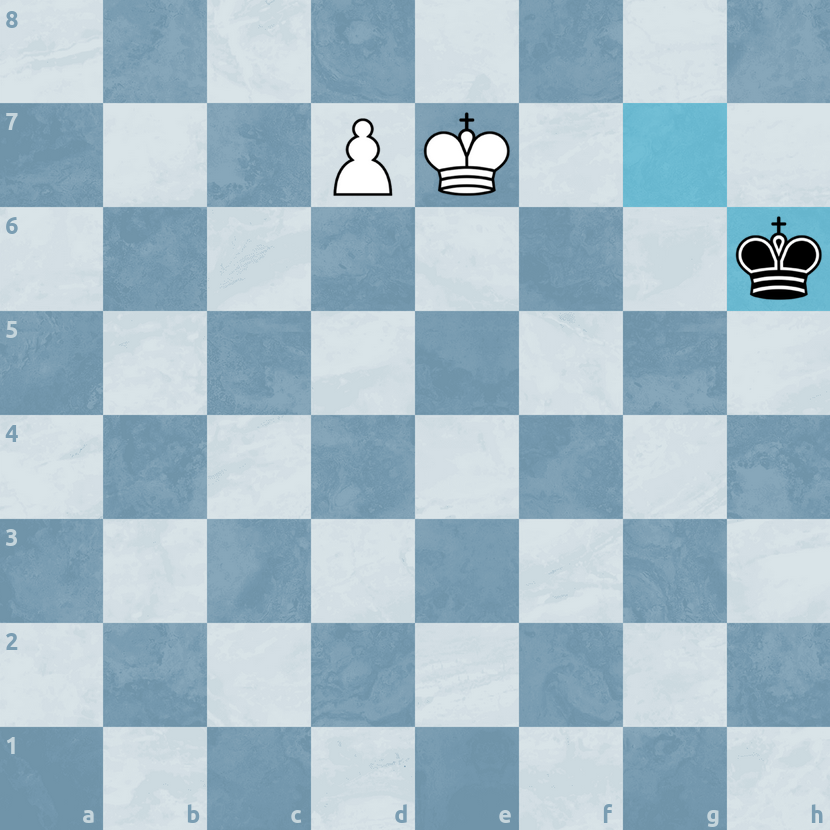
\includegraphics[width=\textwidth, height=\textwidth]{promotion1.png}
     \vspace{0.5cm}
    \textbf{Exemple de promotion}
 \end{minipage}
 \hfill
 \begin{minipage}{0.48\textwidth}
     \centering
     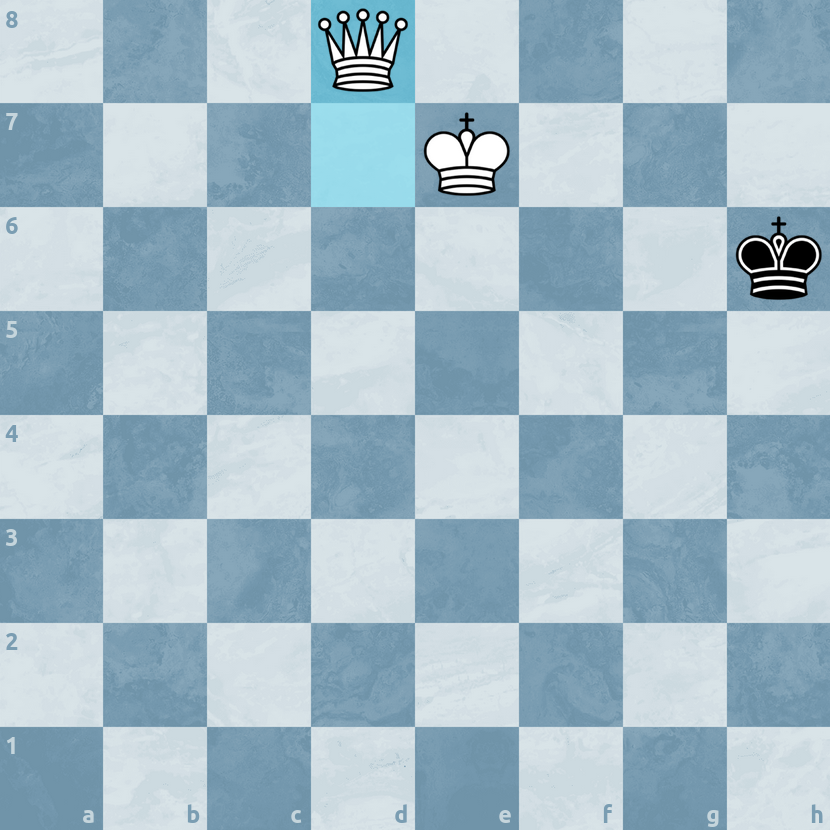
\includegraphics[width=\textwidth, height=\textwidth]{promotion2.png}
     \vspace{0.5cm}
 \end{minipage}

\subsubsection{Fin de Partie}
Une partie d'échecs peut se terminer de plusieurs façons :
\begin{itemize}
    \item \textbf{Échec et mat} : le roi est attaqué et aucun coup légal ne peut le sauver, ce qui donne la victoire à l'adversaire.
    \item \textbf{Pat} : un joueur n'a aucun coup légal à jouer et son roi n'est pas en échec, entraînant une nulle.
    \item \textbf{Manque de matériel} : si seuls les rois, ou un roi et un fou/cavalier, restent sur l'échiquier, un mat devient impossible, ce qui entraîne une nulle.
    \item \textbf{Répétition de position} : une même position exacte apparaît trois fois, entraînant une nulle.
    \item \textbf{Règle des 50 coups} : si aucun pion n'est déplacé ni pièce capturée pendant 50 coups consécutifs, la partie est déclarée nulle.
    \item \textbf{Abandon} : un joueur peut décider d'abandonner si sa position devient trop défavorable.
    \item \textbf{Accord mutuel} : les deux joueurs conviennent de déclarer une nulle lorsqu'aucun ne voit de progrès réaliste possible.
    \item \textbf{Dépassement de temps} : un joueur perd si son chronomètre s'écoule avant qu'il ne joue, sauf si l'adversaire n'a pas assez de matériel pour mater.
\end{itemize}

\subsection{Plateau sous forme de bitmaps}
Un échiquier est finalement une matrice 8x8 (64 cases donc) sur lesquelles il y a une pièce, ou non. On voit ici une
notion de binaire. Pour une pièce: "Blanche ou Noire", "Présente ou Non" (pour les cases). Une méthode existe pour
représenter l'échiquier en se servant de bitmaps plutôt que d'utiliser des arrays, vecteurs ou listes en deux dimensions.
Il s'agit du bitboard. On observera un gain de performance en temps et un gain d'espace énormes pour la représentation
de l'échiquier (et des règles spécifiques).\\
Comment cela va-t-il fonctionner ? Comme on vient de le voir, sur une case, soit il y a une pièce, soit il n'y en a pas.
Encodons le fait qu'une case soit occupée par 1 et le fait qu'une case soit vide (libre) par 0. Il y a 64 cases au total.
Donc, en attribuant un indice à chaque case (de 0 à 63), on va pouvoir chiffrer l'échiquier par un entier de 64 bits.
Chaque bit de cet entier est à 0 ou à 1. S'il est à 0 pour l'indice i, alors la case i est libre. S'il est à 1, alors la
case i est occupée. Un entier n'est cependant pas suffisant, car il faut pouvoir différencier les types de pièce, ainsi
que la couleur des pièces (noire ou blanche). Il y a au total 6 types de pièces aux échecs: le Pion, le Cavalier, le Fou,
la Tour, la Dame, le Roi. Donc finalement, on aura besoin de 12 entiers codés sur 64 bits, car 6 pour les types de pièces
blanches et 6 pour les types de pièces noires.
\\Il est important de noter que cela n'est pas réalisable pour des ordinateurs qui possèdent une architecture en 32 bits.
Aujourd'hui, la quasi-totalité des ordinateurs utilise du 64 bits, donc il ne faut pas trop s'en soucier. C'est néanmoins
crucial de relever les inconvénients des méthodes que l'on va utiliser pour ce projet. Un autre désavantage de cette méthode
est le fait qu'il faudra faire une gymnastique pour "décoder" pour l'humain une position. En effet, si l'on prend l'entier
112, on ne visualise pas (du tout) la position, même si l'ordinateur si.
Retenons aussi que l'on aura à faire à des représentations et opérations binaires, pour lesquelles un ordinateur est très
performant. En Java, chaque entier sera un long (type primitif).
\\Il faut aussi se pencher sur les règles spécifiques que l'on encodera avec les 12 bitmaps pour représenter une position
dans son entièreté. Effectivement, pour le moment, nous n'avons que l'emplacement des pièces sur l'échiquier. Mais une position
est aussi décrite par ses règles, c'est un état de jeu. Les règles à prendre en compte sont:\\
\begin{itemize}
    \item En passant: Il faut utiliser 1 bit comme flag, 1 si en passant possible et 0 sinon. Il y a au total 16 cases cibles où
    un en passant peut se produire. On utilise donc 4 bits (16 valeurs) supplémentaires. Au total donc, 5 bits.
    \item Roques: on compte le grand roque et le petit roque des deux côtés (noirs et blancs). On a donc besoin de 4 bits.
    \item Temps à la pendule: Pour les blancs et les noirs, on doit savoir combien de temps il reste à chaque état du jeu. Si
    l'on se dit que chaque joueur dispose de 24h pour une partie en prenant large, il faut coder 86 400 000 (en ms). Pour cela,
    on a besoin de 27 bits. Mais il s'agit de 27 bits de chaque côté car il y a les blancs et les noirs. Donc au total, 54 bits ici.
    \item Règle des 50 coups: Pour le nombre de coups sans capture ou mouvement de pion, on se sert de 6 bits (entre 0 et 50).
    \item Nombre de "FullMoves": Pour se souvenir du nombre de coups total de la partie, on va prendre large et utiliser 10 bits,
    ce qui nous donne la possibilité d'avoir 1000 coups.
\end{itemize}

Si l'on effectue le total, une position est codée sur 12*64 + 5 + 4 + 54 + 6 + 10 = 847 bits.
C'est un gain très conséquent qui va notamment nous permettre par exemple de chercher à une profondeur plus grande pour la partie
Intelligence Artificielle. Il y a quelques détails en ce qui concerne les performances dans les parties \ref{DataStruct} Structures de données et
\ref{AI} Intelligence Artificielle dans le rapport notamment.

\subsection{Structures de données}
\label{DataStruct}
\subsubsection{Historique des coups}
\par Le groupe s'est posé la question de quelles structures de données utiliser pour stocker l'historique des coups d'une
partie. Il a fallu prendre en compte plusieurs facteurs, notamment la performance, la ou les difficultés d'implémentation,
la compatibilité avec les bitboards pour représenter le plateau de jeu, ainsi que les ajouts potentiels de fonctionnalités.
\\La première idée fut une pile. En effet, cette structure est très simple d'utilisation et parfaitement adaptée pour stocker
des coups, tout en ayant la possibilité d'en enlever et d'en rajouter. La complexité en temps et en espace est en O(n) si n 
correspond au nombre de coups de la partie. Pour revenir au tout début de la partie, c'est-à-dire avec les pièces positionnées
sur leurs cases initiales, il suffit de dépiler les n coups stackés et les empiler dans une seconde pile qui s'occupera de sauvegarder
ces coups pour pouvoir revenir au dernier coup joué avant d'avoir repris tous les coups. Ainsi, en utilisant la pile comme structure 
de données, on garde n coups en mémoire, et revenir à une certaine position de la partie est linéaire en fonction de ce nombre de coups.
Avec une interface graphique, on pourrait cliquer sur un certain coup pour savoir combien de coups dépiler, car un coup peut arriver
plusieurs fois dans une partie donc sa représentation ne suffit pas. En ce qui concerne le jeu en CLI, il faudrait indiquer le numéro
du coup, ainsi que sa notation pour, encore une fois, savoir combien de coups il faut reprendre.\\
Avec la GUI, cela se présenterait comme ceci (remarquez les coups surlignés en bleu à droite sur les images):

\newpage
\begin{figure}[h]
    \caption{Exemple historique de coups}
    \centering
    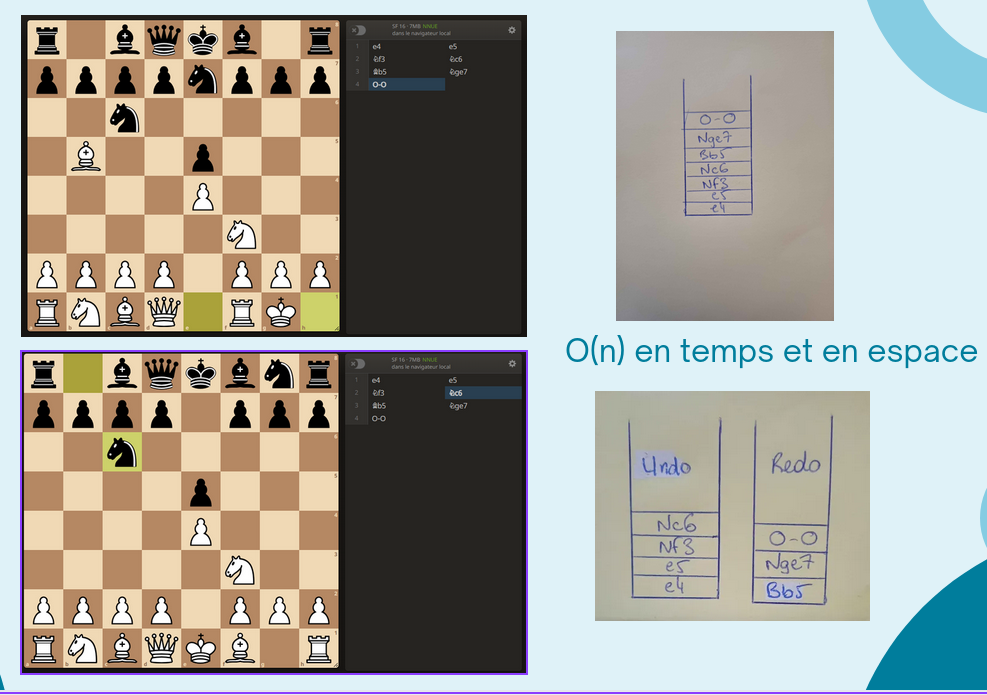
\includegraphics[width=\textwidth,height=7.0cm,keepaspectratio]{pile-historique-coups}
\end{figure}

S'il n'y a pas de fonctionnalité de game review ou de game analysis, et que l'on part du principe qu'il y a écrasement de l'historique
lorsque l'on joue des coups différents de ceux joués initialement, alors la pile est un très bon choix.\\

\par Le groupe a ensuite réfléchi à d'autres structures de données. Rapidement, nous avons noté les listes chaînées, les tableaux,
ainsi que les arbres.
Les listes (doublement) chaînées peuvent être une solution dans certains cas. En effet, l'insertion et la suppression sont des opérations
réalisables en O(1). L'historique est alors plus flexible et les modifications sont assez efficaces. Comme la pile, pour revenir à un
certain coup de la partie, nous sommes en O(n). En revanche, il y a certains cas où cette approche n'est pas très optimale. Par exemple,
pour les parties (très) longues. En effet, la surcharge en mémoire (due aux références) et le coût en temps pour parcourir la liste peuvent
devenir problématiques. Aussi, s'il y a régulièrement un accès à différents coups (précédents comme futurs), cela est moins rapide que des
structures indexées. Finalement, les listes chaînées sont très similaires aux piles sur beaucoup d'aspects (complexité notamment). Cependant,
nous pensons qu'il s'agit d'une solution moins "élégante" et plus "coûteuse" en dette technique et maintenabilité.\\
Nous avons également porté notre attention sur les tableaux, spécialement efficaces pour l'accès à des éléments (O(1)). C'est aussi plutôt
simple et rapide à mettre en oeuvre. Toutefois, on doit avoir une taille fixe pour cela. Ou alors, il faudrait effectuer des réallocations,
qui peuvent devenir coûteuses sur le long terme. De même, pour réécrire l'historique, cela peut prendre O(n) en temps, sans compter que
l'espace mémoire a pu être alloué "pour rien" au sens où l'on aurait au bout du compte pas eu besoin d'autant de mémoire.\\
Finalement, les arbres auraient aussi pu être intéressants dans le cas où il y aurait des variations (branchement), car ils offrent une complexité
assez valable en temps. En effet, lorsque l'on déroule les branches ou variations de coups,
l'arbre est en fait la structure de données naturelle dont on va se servir. C'est d'ailleurs ce que l'IA utilisera dans le cadre de la recherche
du meilleur coup.\\
Remarquons que sans les branchements (dans notre cas donc), utiliser un arbre revient à utiliser une liste chaînée.
Regardons un exemple pour ensuite discuter les avantages et les inconvénients des arbres:\\
\begin{center}
    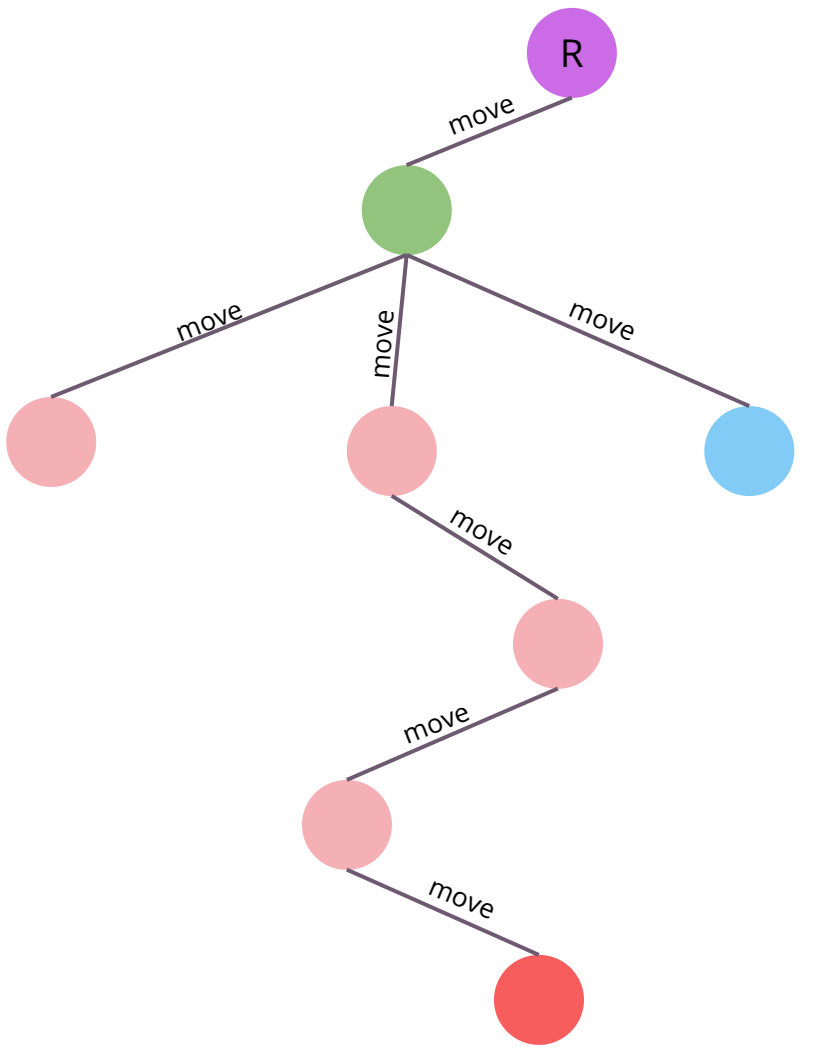
\includegraphics[height=6.0cm]{arbres-branchement-coups.png}
\end{center}

Dans notre exemple, les nœuds représentent les positions
et les arêtes représentent les coups. Si l'on est au nœud rouge, et que l'on souhaite revenir au nœud vert pour aller vers le nœud bleu,
alors la nouvelle branche "main" pour l'historique des coups va du nœud R (Root) jusqu'au nœud bleu. Avant, il allait du nœud R jusqu'au
nœud rouge. \'A chaque nœud de branchement (ici nœud vert), on aurait la possibilité de changer de branche. C'est-à-dire que si l'on revient
au nœud vert, on pourrait retourner au nœud bleu, comme on pourrait retourner au nœud rouge, ou comme on pourrait explorer d'autres coups,
créant ainsi une nouvelle variation depuis ce nœud de branchement.

En terme de performance, au niveau de la complexité en temps, cela serait imbattable, car on pourrait revenir à une position en O(1) (noeuds de branchement).
En effet, en se servant d'une Java HashMap\textless Integer, Node\textgreater. On obtiendrait ainsi une référence à partir d'un entier en se servant de
l'interface graphique (valable seulement pour la GUI):\\
\begin{center}
    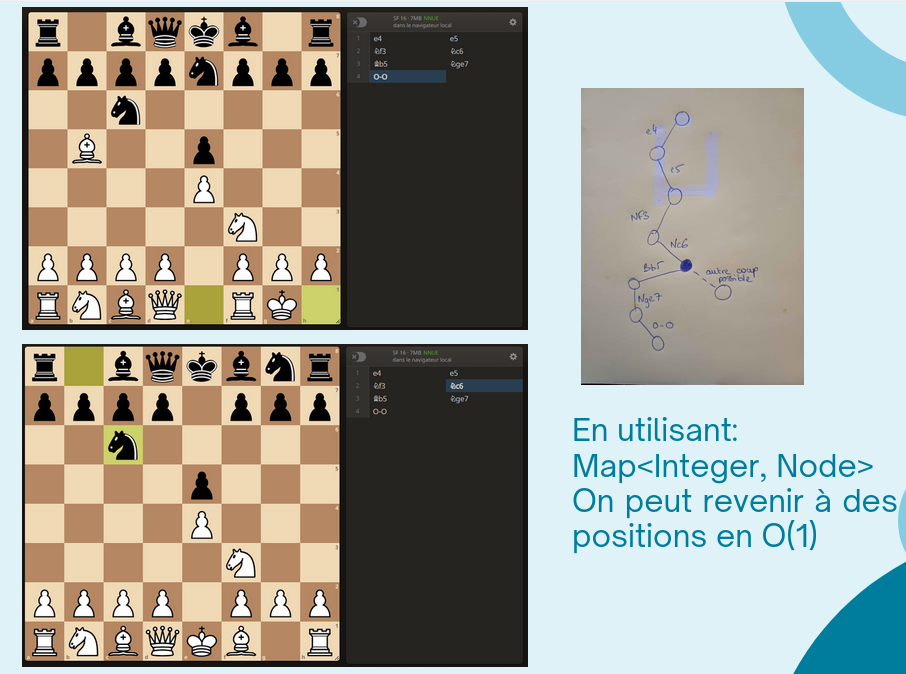
\includegraphics[height=6.0cm]{arbres-reprise-coups.png}
\end{center}


En ce qui concerne la complexité en espace, cela devient un petit peu plus délicat si l'on souhaite être précis. Avant tout, pour permettre de
revenir dans l'ordre en O(1), il faut conserver toutes les références des nœuds de cet arbre. Cela signifie que l'on garde en mémoire n+1 positions 
si n est le nombre de coups joués au total (branches comprises). Comme nous l'avons vu précédemment, une position est encodée par 847 bits.
Finalement, on se retrouve avec une complexité de O(847*n) bits. Pour donner un ordre d'idée, si une partie a enregistré 300 coups, alors en mémoire,
on aura un peu moins de 52KB. Ce n'est donc pas très coûteux en ce qui concerne une partie. En revanche, pour la partie Intelligence Artificielle,
où l'on va tester des milliers de branchements, cela peut devenir assez lourd. Il faudra certainement faire des tests et limiter les opérations
sur ces arbres de jeu afin de ne pas causer de problème.

\par Nous avons donc observé que les arbres sont de manière générale très avantageux dans le cas de branchement, et bien plus que les piles, pour lesquelles
il aurait fallu faire un nombre indécent de copies et donc coûter cher.
Maintenant, les variations et game reviews sont hypothétiques, donc le groupe préfère ne pas prendre de risque et se servira des piles pour stocker
l'historique des coups d'une partie. Cela est bien plus simple à maintenir et à mettre en oeuvre. Aussi, en ce qui concerne la notation de l'historique
dans les fichiers, cela est plus adapté.

\subsection{Intelligence Artificielle} \label{AI}
\subsubsection{Heuristiques}
Afin de coder une bonne heuristique, aux échecs, il faut prendre en compte beaucoup d'éléments et revenir aux bases du jeu.
Notamment, il faut savoir ce qui importe dans une position, ce qui donne l'avantage ou ce qui assure une égalité. Essentiellement,
on se contente de vérifier certains points clés qui vont nous permettre d'émettre une évaluation sur une position.
Rappelons que le facteur de branchement aux échecs approche les 35.\\
Il y a de nombreux éléments à prendre en compte, et en voici certainement les plus impactants:
\begin{itemize}
    \item Le Matériel: chaque pièce (sauf peut-être le roi) possède une valeur. On va donc s'occuper de compter pour les 2 camps le "potentiel"
    dans une position. Plus on a de matériel (pièces donc), plus on a de chances d'avoir l'avantage, en particulier par un bon contrôle de l'échiquier.
    \item La sécurité du Roi: Le Roi est la pièce la plus importante aux échecs, et souvent, le joueur qui a un avantage est celui qui va
    avoir un Roi qui n'est pas en danger. Pour estimer cela, on peut en particulier vérifier le nombre de coups où l'on peut mettre le Roi en échec,
    combien de coups permettent de l'en sortir, et la fréquence des échecs. Plus un Roi est vulnérable, plus il y aura des possibilités
    de le mettre en échec.
    \item Le contrôle du centre: Aux échecs, le centre est un emplacement clé, puisqu'il peut donner un accès efficace à toutes les parties de
    l'échiquier. Généralement, obtenir un bon contrôle du centre est un facteur qui va jouer dans l'évaluation d'une position.
    \item L'activité: Si l'on a peu de coups légaux que l'on peut jouer, c'est très souvent parce que l'on est en position de désavantage. Cela peut
    signifier que l'on est forcé à jouer certains coups.
    \item La structure de pions: Plus on aura une structure de pions solide, plus on aura de potentiel d'attaque et de défense puisque les pions sont
    des pièces "faibles" lorsqu'ils sont seuls et/ou non défendus.
    \item La promotion: Plus on a de pions avancés, plus on a de chance d'atteindre la dernière rangée et changer notre pion en une pièce plus importante,
    comme la Dame par exemple, nous donnant plus d'options.
\end{itemize}

Seulement ceux-là sont cités ici, mais en réalité, il y a plus de 20 points clés nous permettant d'évaluer une position de manière efficace.
Enfin, afin d'obtenir une bonne heuristique aux échecs, il faut considérer tous ces points et faire une somme. Puisque c'est un jeu à somme nulle,
c'est la marche à suivre. 

\subsubsection{Algorithmes}
Dans cette partie Intelligence Artificielle, on va essentiellement se servir des 3 algorithmes suivants (dont 2 vus au dernier semestre):
\begin{itemize}
    \item MiniMax: Visant à retourner l'option la plus adéquate dans une certaine position, on utilise des arbres pour savoir quelle branche va être la
    plus intéressante, que ce soit pour l'ami, comme pour l'ennemi. On est en O($b^d$) en temps, où b est le facteur de branchement et d la profondeur.
    En espace, c'est du O(d), soit le nombre de niveaux dans l'arbre pour une approche basée sur du DFS.
    \item AlphaBeta-pruning: Cet algorithme se repose sur MiniMax, mais peut permettre d'aller à une profondeur deux fois plus grande si les nœuds de
    l'arbre sont organisés du plus petit au plus grand. Ici, la valeur des nœuds va être une évaluation. La complexité en espace ne change pas, mais
    en temps nous sommes donc en O($b^p$) où p = d/2.
    \item Monte Carlo Tree Search: Celui-ci peut se décomposer en quatres étapes: "Selection",
    "Expansion","Simulation","BackPropagation". Pour faire simple,
    on va choisir (Selection) des branches à explorer. Cela peut être les nœuds qui vont être impactants sur la recherche du meilleur coup,
    ou encore des nœuds qui n'ont pas encore été explorés. Ensuite, après avoir choisi la branche, on se positionne à la feuille de cette branche,
    puis on simule un coup aléatoirement (Expansion) et on l'évalue. Maintenant, à partir de ce nouveau nœud, on simule une partie ou une pseudo-partie
    aléatoirement pour estimer le résultat potentiel. Finalement, lorsque l'on obtient un résultat, on fait remonter l'évaluation (BackPropagation)
    et/ou les informations importantes vers le haut de l'arbre pour plus tard agir en conséquence. En temps, on se rapproche de O(n*d), où n est le
    nombre de simulations effectuées, et d la profondeur moyenne. En espace, on est en O(n*847) où n est le nombre de nœuds au total, et 847 le
    nombre de bits (la taille) d'un nœud.
\end{itemize}

\par Notons que tous les algorithmes s'effectuent sur des arbres et se servent d'une heuristique pour évaluer chaque position. Pour optimiser ces algorithmes, 
on utilisera surtout deux techniques: le Forward-prunig et la Reduction.

\subsection{Zobrist hashing} \label{Zobrist}
Le hachage Zobrist est une fonction utilisée en particulier dans les jeux comme les échecs ou le go, où le but est d'attribuer un codage "complexe" à
une position, pour éviter d'analyser une position plus d'une fois. Ainsi, on peut gagner en performance, notamment dans les algorithmes d'IA, où les
états de jeu peuvent se répéter un grand nombre de fois. On va se servir de ce qu'on appelle des "tables de transposition", qui sont des tables de
hachage indexées par une position. Comment cela fonctionne-t-il ? Dans notre cas, les positions sont encodées par 12 bitmaps, et quelques bits
supplémentaires pour les règles spécifiques. Pour chaque combinaison case-pièce, on va générer un nombre aléatoire. De cette façon, toutes les configurations
de plateaux vont être rencontrées. Le hachage va consister à combiner toutes ces chaînes de bits pour chaque configuration avec l'opérateur XOR,
pour à la fin obtenir un hachage final pour chaque position. Ainsi, en utilisant une HashMap, on va conserver tous les hachages représantant toutes les
configurations possibles pour les utiliser plus tard. Par exemple, pour la règle "Threefold repetition", il faut vérifier si dans cette table de hachage
il existe un hachage H tel que H >= 3. Si c'est le cas, alors la partie se termine en égalité.
\\Donc, dans notre cas, on aura quelque chose de la sorte:\\
\begin{itemize}
    \item ZobristBoardTable[64][12]
    \item ZobristEnPassantTable[64]
    \item ZobristCastlingRightsTable[16]
    \item ZobristFiftyMoveRuleTable[51]
    \item ZobristFullMoveTable[1025]
\end{itemize}

\par Chaque élément sera donc en premier aléatoire, puis bits à bits, des opérations avec XOR seront réalisées. C'est avantageux car lorsque l'on joue
un coup, donc que l'on change l'état du jeu, il n'y a pas à tout recalculer. D'abord, on XOR le nombre aléatoire correspondant à la pièce qui quitte
sa case de départ, puis celui pour la case d'arrivée de cette pièce, et éventuellement changer les bits pour les règles spécifiques.
Pour l'IA, cette méthode sera clé car elle fera gagner en performance, car les états de jeu peuvent se répéter un grand nombre de fois (même si pas
toujours dans le même ordre).

\section{Besoins visés}
\subsection{Quels besoins ?}
Dans le sujet donné, il y avait une liste de 60 besoins.
Nous avons pris la décision ambitieuse de répondre à tous ces besoins. C'est un travail conséquent,
mais avec une équipe de 5 personnes, codant pendant huit semaines,
nous pensons que cet objectif est atteignable.

Nous avons tout de même classé ces besoins par ordre de priorité (voir \nameref{agenda}), afin de garantir
la jouabilité projet même si nous n'arrivons pas à tout implémenter à temps.
Nous voulons rendre un jeu cohérent et fonctionnel avec des modules entièrement
terminés (même s'il en manque) plutôt qu'un projet avec des règles manquantes,
une intelligence artificielle bâclée et une interface graphique peu fonctionnelle.

\subsection{Dépendances entre les besoins}
\subsubsection{Gestion des options}
La première dépendance que nous avons concerne la gestion des options (Figure \ref{fig:needs_options}).

\begin{figure}[h]
    \caption{Besoins concernant la gestion d'options}
    \centering
    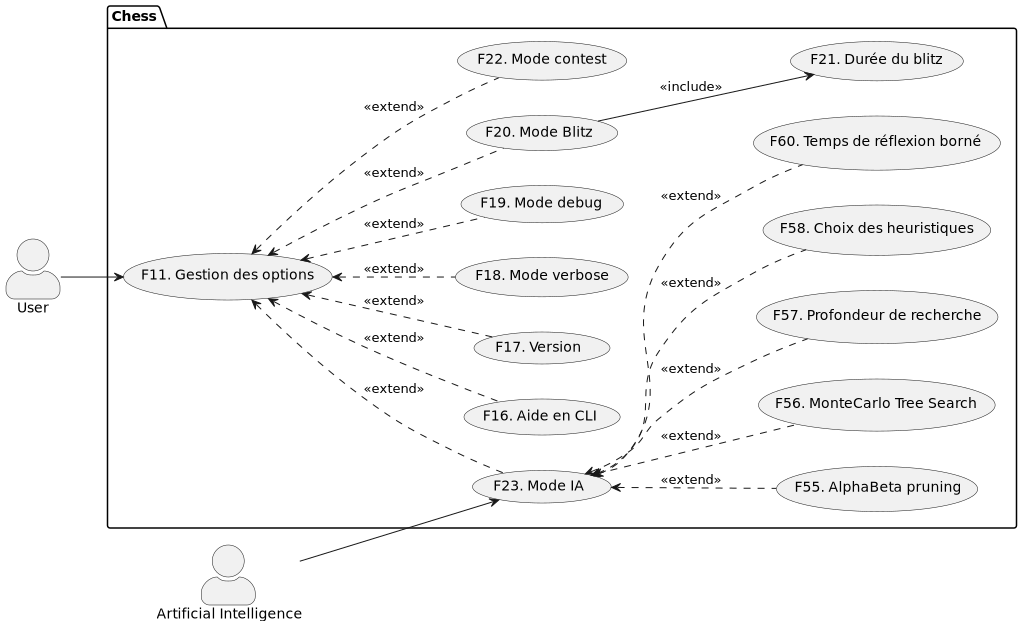
\includegraphics[width=\textwidth,height=\textheight,keepaspectratio]{needs_options}
    \label{fig:needs_options}
\end{figure} 

L'implémentation de la \textit{gestion des options }permettra de rajouter de nombreuses fonctionnalités.
En effet, ceci nous permettra d'implémenter le Mode contest, la version du jeu ou l'aide en ligne de commande. Nous pourrons également gérer les messages affichés grâce au mode verbose ou au mode debug.
Lorsque cela sera implémenté, l'utilisateur aura également le choix entre afficher le jeu en ligne de commande ou avec une interface graphique.
Le mode Blitz inclura le besoin Durée du blitz afin de paramétrer ce mode.
Le mode IA, qui a besoin de la gestion des options, possède quant à lui de nombreuses extensions. En effet, nous pourrons paramétrer
notre intelligence artificielle grâce à d'autres options, que nous verrons cela plus en détail à la section \ref{IA}.


\subsubsection{Sauvegarde de l'historique}
La gestion de l'historique est un besoin indispensable pour notre jeu (Figure \ref{fig:needs_files}).
Beaucoup de besoins dépendent de cette fonctionnalité.
\begin{figure}[h]
    \caption{Besoins concernant la sauvegarde de l'historique}
    \centering
    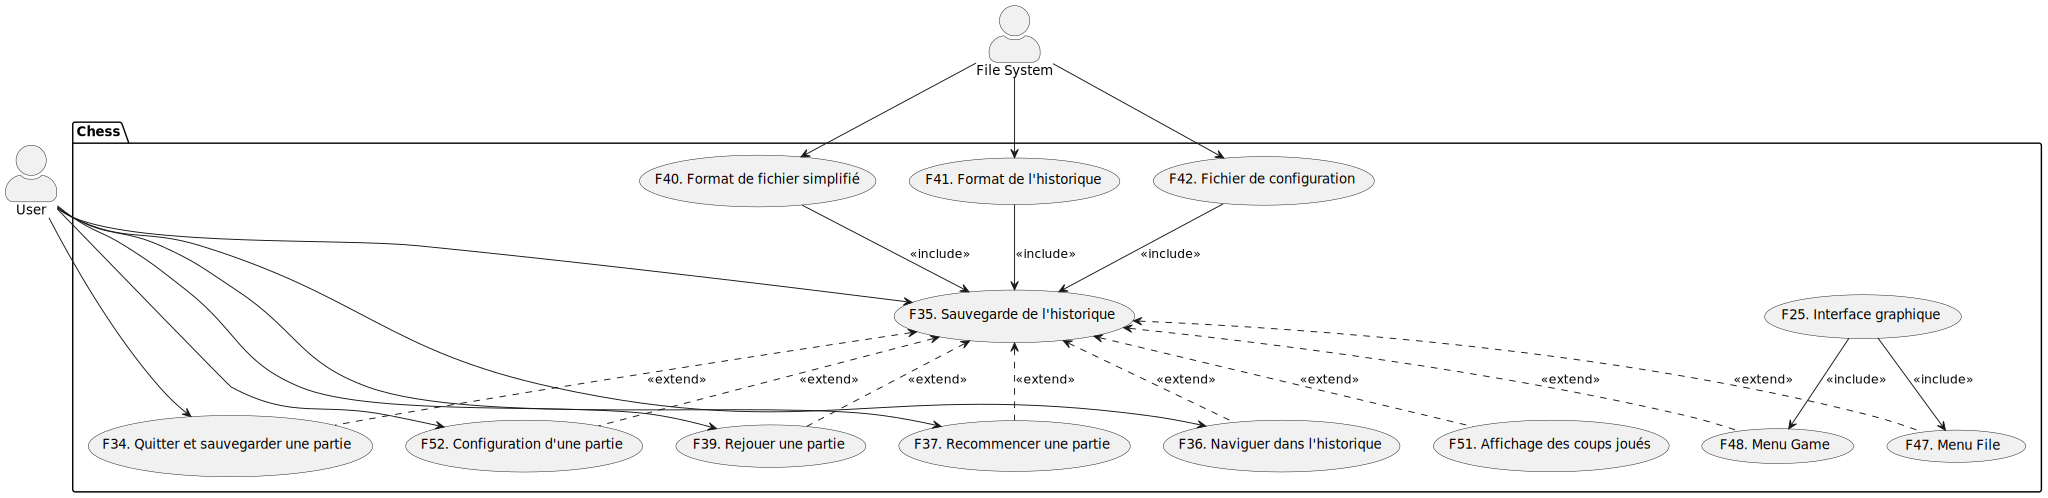
\includegraphics[width=\textwidth,height=\textheight,keepaspectratio]{needs_files}
    \label{fig:needs_files}
\end{figure}

Avant de pouvoir implémenter la gestion de l'historique, il faudra d'abord choisir les formats de fichiers.
Pour cela, il faudra remplir les besoins suivants: \textit{Format de fichier simplifié}, \textit{Format de l'historique} et \textit{Fichier de Configuration}.
Une fois ces besoins implémentés, la sauvegarde de l'historique sera donc possible.
Des besoins utiles au bon déroulement du jeu en dépendent. Grâce à cela, l'utilisateur pourra sauvegarder
sa partie, rejouer ou recommencer une partie. Il pourra également configurer sa partie en modifiant les données du fichier de configuration.
Cela permettrait aussi d'afficher les coups précédemment joués, et même de remonter dans l'historique pour annuler un coup et revenir en arrière.
Certains menus de l'interface graphique permettront également de gérer ces fichiers de sauvegarde et de configuration (voir figure \ref{fig:needs_gui}).

\subsubsection{Intelligence artificielle}
\label{IA}
L'implémentation d'une intelligence artificielle est un autre besoin central du jeu. En effet, cela pourra
permettre à l'utilisateur de jouer contre une machine. Cela pourrait également permettre de donner des
indications sur les meilleurs coups à jouer pour le joueur.

\begin{figure}[h]
    \caption{Besoins concernant l'intelligence artificielle}
    \centering
    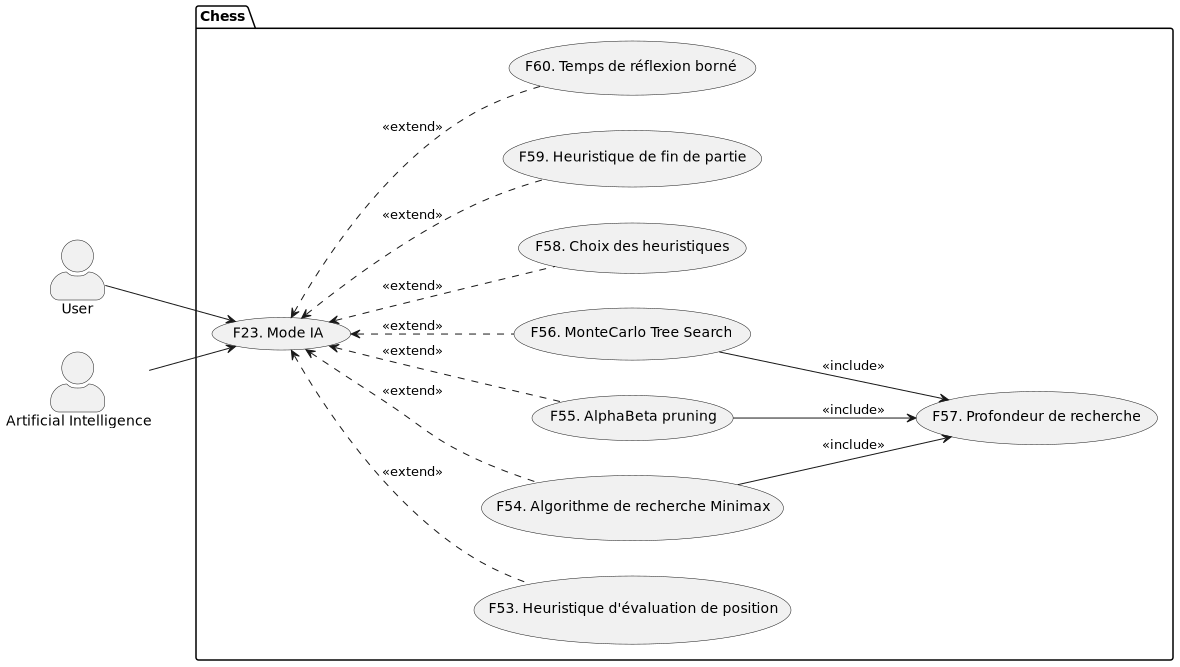
\includegraphics[width=\textwidth,height=\textheight,keepaspectratio]{needs_ai}
    \label{fig:needs_ai}
\end{figure}

Comme affiché Figure \ref{fig:needs_ai}, nous pouvons voir que de nombreux besoins
concernent l'intelligence artificielle.
La plupart des besoins affichés sont également présent dans la Figure \ref{fig:needs_options}, car ils sont paramétrables
en ligne de commande.
Le mode IA contient différentes fonctionnalités concernant les heuristiques. Nous devons implémenter différentes \textit{heuristiques}
d'évaluation de position, mais également au moins une heuristique de fin de partie. Ces heuristiques permettront "d'aider" le joueur IA
à jouer. Ces heuristiques pourront être utilisées avec l'\textit{algorithme de recherche Minimax} mais également lors de l'\textit{AlphaBeta pruning} 
et le \textit{Monte Carlo Tree Search}. Ces algorithmes dépendent tous de l'option \textit{Profondeur de recherche}. En effet, le jeu des échecs est bien 
trop complexe pour simuler une partie entière, et nous devons nous limiter à une certaine profondeur de recherche (nombre de coups à jouer puis analyser).
Borner le temps de "réflexion" de l'IA est aussi un moyen de limiter les calculs de ces algorithmes. Cela pourrait permettre à l'utilisateur de jouer une partie contre
un joueur IA plus ou moins efficace ou d'attendre plus ou moins longtemps entre ses tours.
\subsubsection{Interface graphique}
Les derniers besoins que nous avons rassemblés sont ceux concernant l'interface graphique (Figure \ref{fig:needs_gui}).
\begin{figure}[h]
    \caption{Besoins concernant l'interface graphique}
    \centering
    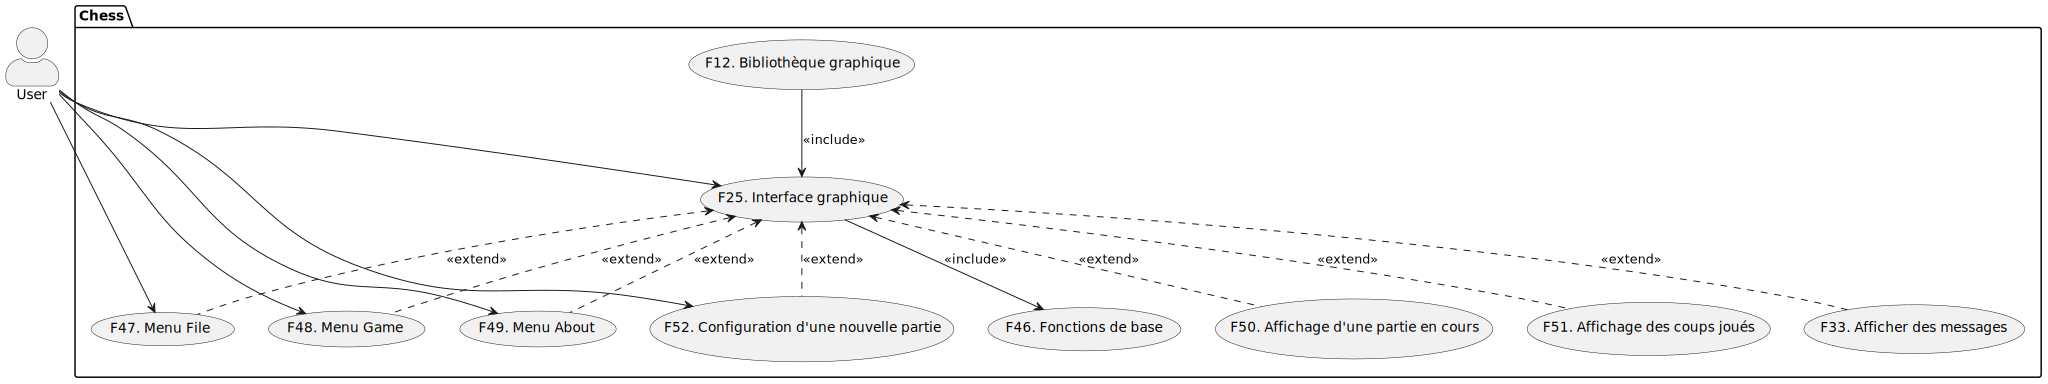
\includegraphics[width=\textwidth,height=\textheight,keepaspectratio]{needs_gui}
    \label{fig:needs_gui}
\end{figure}

L'interface graphique dépend de la \textit{bibliothèque graphique} choisie, ici elle est imposée, il s'agit de \textit{JavaFX}.
L'utilisateur peut choisir de l'utiliser grâce aux options en ligne de commande (Figure \ref{fig:needs_options}).
Elle doit permettre d'utiliser les fonctions de base que nous avons implémenté pour le jeu en ligne de commande. Nous devons 
pouvoir afficher la partie en cours, les coups joués, ainsi que des messages selon le mode utilisé (Verbose ou Debug, voir figure \ref{fig:needs_options}).
L'utilisateur doit également pouvoir utiliser différents menus afin de pouvoir paramétrer ou sauvegarder sa partie (voir figure \ref{fig:needs_files}) ou obtenir des informations sur le jeu.

\section{Agenda prévisionnel}
\label{agenda}

Nous avons décidé de séparer le temps de programmation en quatre parties. Les trois premières seront rythmées besoin par besoin, et la dernière quant à elle sera dédiée à la finalisation du projet et la préparation d'un livrable.
Une partie des besoins sera également suivie tout au long du projet afin de maintenir une base cohérente.

\subsection{Tout au long du projet}

Gestion des aspects fondamentaux et comme le style de codage, les tests, les performances, et la documentation pour garantir la cohérence et la qualité globale du code.

\begin{itemize}
    \item F1. Langage de programmation
    \item F2. Style de codage
    \item F3. Langue par défaut dans le code
    \item F4. Système cible
    \item F5. Documentation
    \item F6. Tests
    \item F10. Frameworks de tests
    \item F7. Bugs
    \item F8. Performances
    \item F9. Build-system
    \item F14. Nom de l'exécutable principal
    \item F15. Usage général
\end{itemize}

\subsection{Semaines 0-2}

Mise en place des fonctionnalités essentielles pour le jeu en ligne de commande, telles que la gestion des options CLI, les règles de jeu, et l'affichage de l'échiquier.

\begin{itemize}
    \item \textbf{Options CLI :}
    \begin{itemize}
        \item F11. Gestion des options
        \item F16. Aide en ligne de commande
        \item F17. Version
        \item F18. Mode verbose
        \item F19. Mode debug
        \item F13. Internationalisation
    \end{itemize}
    \item \textbf{Gestion du jeu :}
    \begin{itemize}
        \item F43. Plateau de jeu
        \item F44. Module bitboard
        \item F45. État du jeu
    \end{itemize}
    \item \textbf{Règles :}
    \begin{itemize}
        \item F29. Prise en passant
        \item F30. Roque
        \item F31. Promotion du pion
        \item F38. Fin de partie
    \end{itemize}
    \item \textbf{Jeu CLI :}
    \begin{itemize}
        \item F24. Interface en ligne de commande
        \item F26. Affichage de l'échiquier
        \item F27. Notation des coups
        \item F28. Représentation de l'historique
        \item F33. Affichage des messages
    \end{itemize}
\end{itemize}

\subsection{Semaines 2-4}

Développement de l'IA, avec des algorithmes comme Minimax et Monte Carlo, et ajout de fonctionnalités avancées comme la sauvegarde, la navigation dans l'historique, et le fichier de configuration.

\begin{itemize}
    \item \textbf{IA :}
    \begin{itemize}
        \item F23. Mode IA
        \item F53. Heuristique d'évaluation de position
        \item F54. Algorithme de recherche Minimax
        \item F55. $\alpha\beta$-pruning
        \item F56. Monte Carlo Tree Search
        \item F57. Profondeur de recherche
        \item F59. Heuristique de fin de partie
        \item F60. Temps de réflexion borné
    \end{itemize}
    \item \textbf{Fonctionnalités :}
    \begin{itemize}
        \item F32. Abandon
        \item F34. Quitter et sauvegarde une partie
        \item F35. Sauvegarde de l'historique
        \item F36. Naviguer dans l'historique
        \item F37. Recommencer une partie
        \item F40. Format de fichier simplifié
        \item F41. Format de l'historique
        \item F42. Fichier de configuration
    \end{itemize}
\end{itemize}

\subsection{Semaines 4-6}

Création de l'interface graphique et finalisation des fonctionnalités utilisateurs, incluant les menus interactifs, la gestion des parties, et les modes spéciaux comme le mode blitz et contest.

\begin{itemize}
    \item \textbf{Interface graphique :}
    \begin{itemize}
        \item F12. Bibliothèque graphique
        \item F25. Interface graphique
        \item F46. Fonctions de base
        \item F47. Menu 'File'
        \item F48. Menu 'Game'
        \item F49. Menu 'About'
        \item F50. Affichage d'une partie en cours
        \item F51. Affichage des coups joués
        \item F52. Configuration d'une nouvelle partie
    \end{itemize}
    \item \textbf{Fonctionnalités :}
    \begin{itemize}
        \item F20. Mode blitz
        \item F21. Durée du blitz
        \item F22. Mode contest
        \item F39. Rejouer une partie
        \item F58. Choix des heuristiques
    \end{itemize}
\end{itemize}



Le diagramme de Gantt ci-dessous schématise notre agenda prévisionnel, avec les sous-besoins détaillés. 
Pour plus d'informations voir la section \ref{Spec}. Nous avons réparti les besoins par personnes,
chacun avec une couleur différente. Si une tâche est moins/plus longue que prévue, nous reverrons la distribution
pour la rendre plus égale.

\begin{center}
    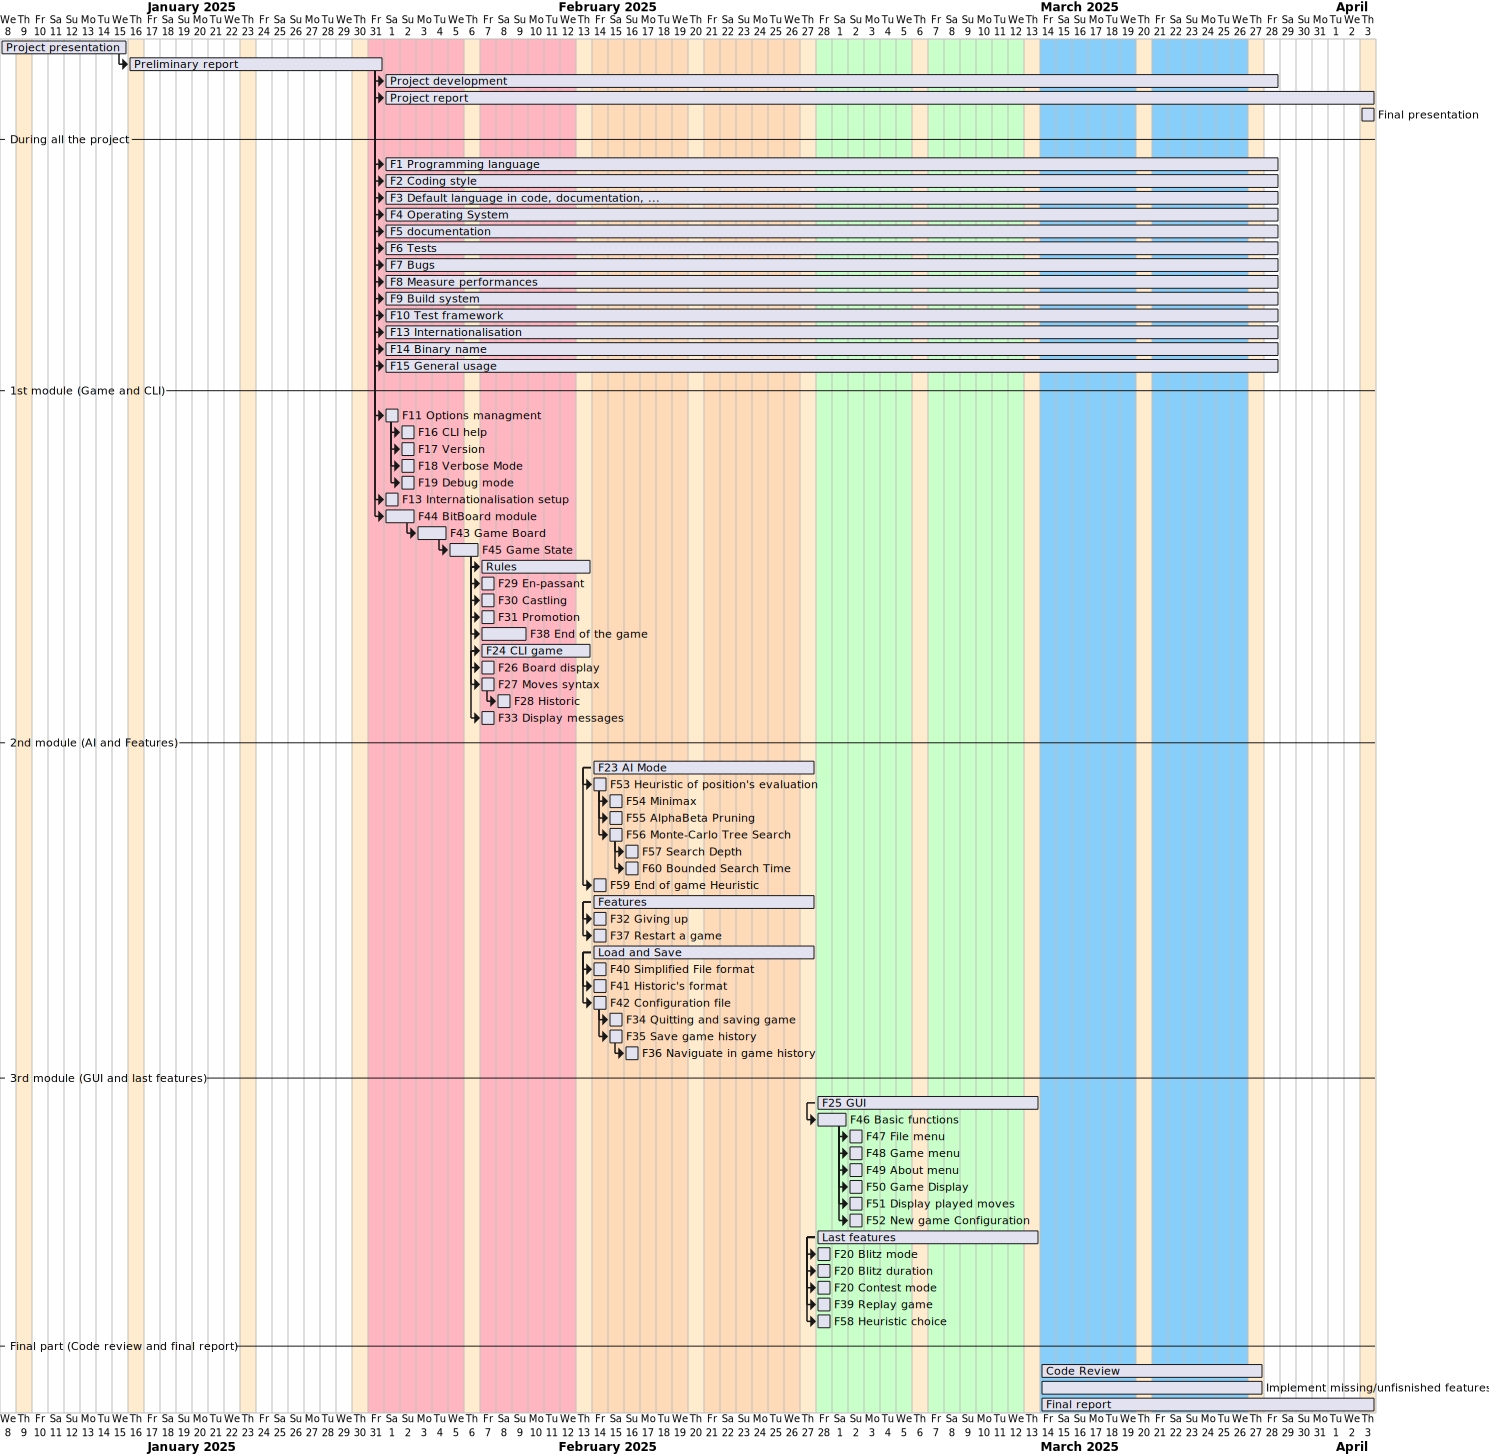
\includegraphics[width=\textwidth,height=\textheight,keepaspectratio]{gantt}
\end{center}

\section{Architecture visée pour le projet}
Nous avons décidé de présenter le projet sous une forme d'architecture MVC personnalisée. Cette architecture est particulièrement pratique pour nous, développeurs, aussi bien en termes de maintenance que pour l'amélioration future du projet.

Les différents modules de notre projet sont les suivants : \textbf{Model}, \textbf{Controller}, \textbf{Vue}, \textbf{Events} et \textbf{Utils}. 

Voici l'architecture UML du projet : 

\begin{center}
    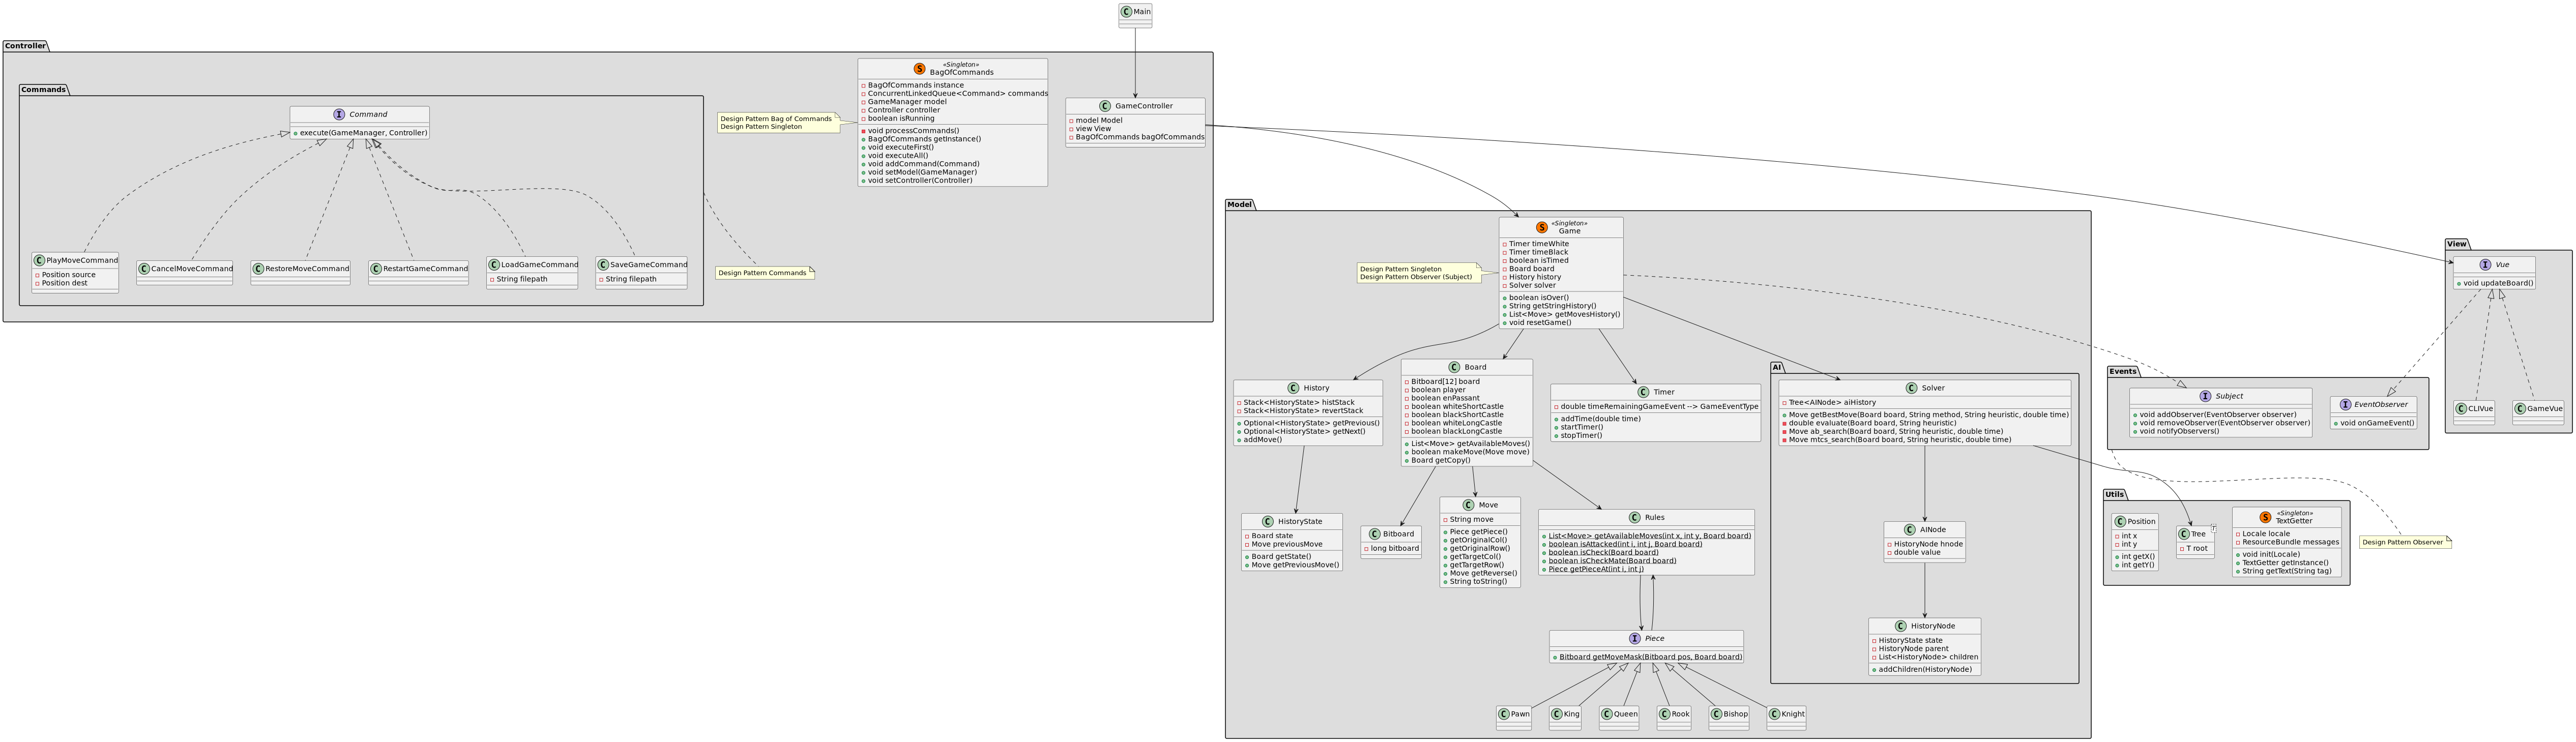
\includegraphics[width=\textwidth,height=\textheight,keepaspectratio]{archiUML}
\end{center}




\subsubsection{Description des Modules}

\begin{itemize}
    \item \textbf{Model} : Gère la logique métier du jeu, incluant l'état de la partie, les règles d'échecs et les fonctionnalités comme l'historique et le timer.
    \item \textbf{Controller} : Sert d'intermédiaire entre la Vue et le Model. Il gère les événements utilisateurs et orchestre les interactions entre les différentes couches.
    \item \textbf{Vue} : Responsable de l'affichage et des interactions avec l'utilisateur, qu'il s'agisse d'une interface CLI ou graphique.
    \item \textbf{Events} : Implémente un système d'observateurs pour gérer les notifications et la communication asynchrone entre les modules.
    \item \textbf{Utils} : Contient des outils génériques comme le gestionnaire de textes internationalisés (\texttt{TextGetter}) et les algorithmes d'intelligence artificielle pour le jeu.
\end{itemize}

\subsubsection{Design Patterns Utilisés}

Les différents design patterns utilisés dans ce projet sont les suivants : 
\begin{itemize}
    \item \textbf{Singleton} : Utilisé pour le module \texttt{Utils/TextGetter} afin de centraliser l'accès aux ressources de texte. Il sera également utilisé pour
la classe \texttt{Game} pour s'assurer qu'une seule instance de game est présente. La classe \texttt{BagOfCommands} utilise ce design pattern afin que la gestion des commandes
ne soit gérée que par un seul bag.
    \item \textbf{MVC} : L'architecture principale du projet, séparant clairement la logique métier, l'affichage et la gestion des événements. C'est un MVC modifié,
 grace au design pattern observer qui va permettre d'envoyer des messages du Model vers la Vue. Cela rend le code plus simple et digeste.
    \item \textbf{Observer} : Permet de notifier la Vue des modifications dans le Model.
    \item \textbf{State} : Utilisé pour gérer l'état de la partie, comme le statut du jeu (en cours, échec et mat, pat, etc.).
    \item \textbf{Command} : Utilisé pour simplifier le Controller. Chaque commande a un objectif précis, effectuer un certain traitement dans le Model.
    \item \textbf{Bag of Commands} : Utilisé pour gérer les Commandes. Nous pourons gérer l'ajout de plusieurs commandes en parallèle.
\end{itemize}


\section{Spécifications étendues}
\label{Spec}

Afin de visualiser au mieux les besoins et sous-besoins que nous avons identifiés, nous les avons présentés comme ci-dessous.
Les encadrés bleus représentent les besoins fonctionnels et on retrouve pour chacun les sous-besoins dans des cadres verts.
Nous utilisons le même principe pour les besoins non fonctionnels (à l'exception que l'encadré est violet). Pour visualiser
au mieux les dépendances entre les besoins, le mieux et de regarder l'agenda prévisionnel (il contient également la répartition
entre les membres du groupe).

\begin{needbox}[F?: Titre]
    Template pour les besoins fonctionnels
    \begin{subneedbox}[F?.?: Titre]
        sous besoin 
    \end{subneedbox}
\end{needbox}

\begin{nonfunctionnalneedbox}[F?: Titre]
    Template pour les besoins non fonctionnels
    \begin{subneedbox}[F?.?: Titre]
        sous besoin
    \end{subneedbox}
\end{nonfunctionnalneedbox}

\subsection{Généralités}

\begin{nonfunctionnalneedbox}[F1. Langage de programmation]
    Le langage de programmation du projet devra être Java et utiliser la spécification Java SE 17+.
\end{nonfunctionnalneedbox}

\begin{nonfunctionnalneedbox}[F2: Style de codage]
    Le coding style du programme doit respecter le coding style de Google.
    \begin{subneedbox}[F2.1: Formattage automatique Iwen]
        Lors du push d'un nouveau commit, appliquer automatiquement le coding style défini.
    \end{subneedbox}
    \begin{subneedbox}[F2.2: Rejet des commits non formatés Iwen]
        Ajouter une étape d'intégration continue vérifiant que le code est correctement formaté.
        Si ce n'est pas le cas, faire échouer la pipeline.
    \end{subneedbox}
\end{nonfunctionnalneedbox}

\begin{nonfunctionnalneedbox}[F3: Langue par défaut dans le code]
    La documentation, le nom des variables, des fonctions et des fichiers devront être en anglais.
\end{nonfunctionnalneedbox}

\begin{nonfunctionnalneedbox}[F4. Système cible]
    Le programme devra fonctionner sur des systèmes d’exploitation GNU/Linux. \\
    \textbf{Test:} Vérifier la compatibilité sur Ubuntu 22.04 et Fedora 36
\end{nonfunctionnalneedbox}

\begin{nonfunctionnalneedbox}[F5. Documentation]
    
    \begin{subneedbox}[F5.1: Option -h]
        Implémenter une option -h (besoin F16).

        \textbf{Prérequis:} F16.

        \textbf{Test:} Vérifier que l'option -h affiche bien l'aide en ligne.
    \end{subneedbox}
    
    \begin{subneedbox}[F5.2: Rédiger un guide utilisateur]
        Rédiger un guide utilisateur pour l'exécutable.

        \textbf{Test:} Vérifier que le guide couvre toutes les fonctionnalités principales.
    \end{subneedbox}
    
    \begin{subneedbox}[F5.3: Ajouter des commentaires au code source]
        Ajouter des commentaires au code source (JavaDoc).

        \textbf{Test:} Vérifier que chaque fonction et classe possède des commentaires explicites.
    \end{subneedbox}
\end{nonfunctionnalneedbox}

\begin{nonfunctionnalneedbox}[F6. Tests]
    Tester et valider le programme avec une couverture suffisante.
    \begin{subneedbox}[F6.1 Tests]
        Implémenter des tests unitaires sur l'ensemble du projet.
    \end{subneedbox}

    \begin{subneedbox}[F6.2 Coverage]
        Les test effectués devront couvrir au minimum 80\% du code.
    \end{subneedbox}
\end{nonfunctionnalneedbox}

\begin{nonfunctionnalneedbox}[F7: Bugs]
    Aucun bug menant à un crash ne doit être présent dans le programme. Les spécifications doivent être respectées et les erreurs doivent générer des messages d'erreur.
\end{nonfunctionnalneedbox}

\begin{nonfunctionnalneedbox}[F8: Performances]
    Evaluer des performances du programme de manière générale et pour différentes options et différentes configurations de jeu
    \begin{subneedbox}[F8.1: IA]
        Estimer précisément les performances de la partie IA, notamment les complexités en temps en en espace en fonction des heuristiques.
    \end{subneedbox}
    \begin{subneedbox}[F8.1: GUI]
        Estimer précisément les performances pour la partie GUI.
    \end{subneedbox}
    \begin{subneedbox}[F8.1: Structures de données]
        Estimer précisément et rendre compte des performances pour la partie structures de données.
    \end{subneedbox}
\end{nonfunctionnalneedbox}

\begin{nonfunctionnalneedbox}[F9: Build-system Iwen]
    Établir un système de build pour le programme avec l'outil Maven pour Java. 
    \begin{subneedbox}[F9.1: Programme seulement]
        Construire un build pour le programme, en écartant les tests et différents autre modes de compilation.
    \end{subneedbox}
    \begin{subneedbox}[F9.2: Tests]
        Construire un build pour les tests (isolés).
    \end{subneedbox}
    \begin{subneedbox}[F9.3: Exécution]
        Construire une commande afin d'exécuter le programme une fois compilé.
    \end{subneedbox}
\end{nonfunctionnalneedbox}

\subsection{Bibliothèques et outils}

\begin{nonfunctionnalneedbox}[F10. Frameworks de test Iwen]
    Tester le code avec des frameworks donnés afin d'avoir un code sans bugs.
    \begin{subneedbox}[F10.1 Utiliser JUnit]
        Implémenter des tests unitaires.
    \end{subneedbox}

    \begin{subneedbox}[F10.2 Utiliser Jacoco pour la couverture de code]
        Vérifier la couverture de code régulièrement pour maintenir les 80\% de couverture
    \end{subneedbox}
\end{nonfunctionnalneedbox}

\begin{nonfunctionnalneedbox}[F11. Gestion des options Mathilde]
    La gestion des options sera basée sur la bibliothèque \textit{commons-cli}.
\end{nonfunctionnalneedbox}

\begin{nonfunctionnalneedbox}[F12: Bibliothèque graphique Iwen]
    La bibliothèque graphique utilisée sera basé sur JavaFx
    \begin{subneedbox}[F12.1: Mise en place d'un environnement de test]
        Mettre en place TestFx afin de pouvoir tester l'interface graphique
    \end{subneedbox}
\end{nonfunctionnalneedbox}

\begin{nonfunctionnalneedbox}[F13: Internationalisation Mathilde]
    Le framework d'internationalisation sera basé sur ResourcesBundle et Locale.
    \begin{subneedbox}[F13.1: Accessibilité du changement de langue]
        Le changement de langue doit pouvoir être effectué en seulement 3 cliques
        sur l'interface graphique.
    \end{subneedbox}
\end{nonfunctionnalneedbox}

\subsection{Options en ligne de commande}

\begin{nonfunctionnalneedbox}[F14. Nom de l’exécutable principal Mathilde]
    L’exécutable principal doit s’appeler "chess" et permettre de lancer tout le programme.
    \textbf{Test:} Vérifier que le programme se lance correctement avec le nom 'chess'.
\end{nonfunctionnalneedbox}

\begin{needbox}[F15. Usage général]
    \begin{subneedbox}[F15.1: Forme et nom du programme Mathilde]
        Le programme devra s’appeler chess et devra s'exécuter de la manière suivante :  
        \texttt{\#> chess [OPTIONS] [FILENAME]}

        \textbf{Test:} Vérifier que le programme se lance correctement avec les options spécifiées.
    \end{subneedbox}
    
    \begin{subneedbox}[F15.2: Gestion des options en ligne de commande Mathilde]
        Vérifier si les options sont correctes. En cas d'erreur, afficher un message d'erreur (stderr) et l’aide en ligne de commande -h.

        \textbf{Prérequis:} F5.1.

        \textbf{Test:} Tester différentes combinaisons d'options valides et invalides.
    \end{subneedbox}
    
    \begin{subneedbox}[F15.3: Démarrage/Chargement d’une partie à partir d’un fichier]
        Si un nom de fichier est donné, charger depuis le fichier. Sinon, démarrer une nouvelle partie avec les options par défaut.

        \textbf{Test:} Vérifier le comportement avec et sans fichier en paramètre.
    \end{subneedbox}
    
    \begin{subneedbox}[F15.4: Gestion des sorties standard et des erreurs]
        Les messages d’erreurs doivent être affichés sur stderr et les messages utilisateur sur stdout.

        \textbf{Test:} Simuler des erreurs et vérifier les messages sur les sorties appropriées.
    \end{subneedbox}
    
    \begin{subneedbox}[F15.5: Codes de retour du programme]
        Le code de retour devra être EXIT\_SUCCESS en cas de succès et EXIT\_FAILURE en cas d’erreur.

        \textbf{Test:} Tester les retours en cas de paramètres valides et invalides.
    \end{subneedbox}
\end{needbox}

\begin{needbox}[F16: Aide en ligne de commande Mathilde]
    L'option '-h', '--help' affiche l'aide puis quitte.

    \textbf{Prériquis:} F11
    \begin{subneedbox}[F16.1: Texte]
        Rédaction du message d'aide destiné à l'utilisateur.
    \end{subneedbox}
    \begin{subneedbox}[F16.2: Affichage]
        Affichage du message d'aide lorsque l'option \textit{-h} ou \textit{--help} est utilisée.\\
        \textbf{Test:} Vérifier que le message d'aide s'affiche.
    \end{subneedbox}
    \begin{subneedbox}[F16.3: Quitter]
        Quitter le programme après l'affichage effectué.\\
        \textbf{Test:} Le programme doit se fermer avec un code de sortie EXIT\_SUCCESS.
    \end{subneedbox}
\end{needbox}

\begin{needbox}[F17: Version Mathilde]
    L'option '-V', '--version' affiche la version puis quitte.

    \textbf{Prériquis:} F11
    \begin{subneedbox}[F17.1: Texte]
        Rédaction du message de version actuelle.
    \end{subneedbox}
    \begin{subneedbox}[F17.2: Affichage]
        Affichage du message de version lorsque l'option \textit{-V} ou \textit{--version} est utilisée.\\
        \textbf{Test:} Vérifier que le message de version s'affiche.
    \end{subneedbox}
    \begin{subneedbox}[F17.3: Quitter]
        Quitter le programme après l'affichage effectué.\\
        \textbf{Test:} Le programme doit se fermer avec un code de sortie EXIT\_SUCCESS.
    \end{subneedbox}
\end{needbox}

\begin{needbox}[F18: Mode verbose Mathilde]
    Réalisation d'un mode verbose, rapportant certaines informations supplémentaires au(x) joueur(s).\\
    \textbf{Test:} S'assurer que toutes les informations sont apportées aux joueurs lorsque l'option
    verbose est choisie.\\
    \textbf{Prériquis:} F11
    \begin{subneedbox}[F18.1: Temps par coup]
        Indiquer à l'utilisateur le temps qui a été pris par un des côtés pour jouer le dernier coup.
    \end{subneedbox}
    \begin{subneedbox}[F18.2: Evaluation de la postion contre l'IA]
        Indiquer à l'utilisateur qui des noirs ou des blancs a l'avantage (s'il y a avantage).
    \end{subneedbox}
    \begin{subneedbox}[F18.3: Moment de la partie]
        Indiquer à l'utilisateur si l'on se trouve plutôt en début, milieu, ou fin de partie.
    \end{subneedbox}
    \begin{subneedbox}[F18.4: Règles spécifiques]
        Indiquer à l'utilisateur les règles spécifiques encore possibles pour chaque état de la partie.
    \end{subneedbox}
\end{needbox}
    
\begin{needbox}[F19: Mode debug Mathilde]
    Réalisation d'un mode debug, rapportant aux développeurs certaines informations sur le programme.\\
    \textbf{Test:} S'assurer que toutes les informations sont apportées aux développeurs lorsque l'option
    debug est choisie.\\
    \textbf{Prériquis:} F11
    \begin{subneedbox}[F19.1: Etat de la partie]
        Indiquer aux développeurs la représentation de chaque position, avec les bitmaps et chaînes de bits pour les
        règles spécifiques.
    \end{subneedbox}
    \begin{subneedbox}[F19.2: Structures de données]
        Indiquer aux développeurs l'état des structures de données à tout moment, en particulier le contenu de la pile pour chaque position.
    \end{subneedbox}
    \begin{subneedbox}[F19.3: Zobrist hashing]
        Indiquer aux développeurs s'il y a des collisions en ce qui concerne le hashing des positions.
    \end{subneedbox}
    \begin{subneedbox}[F19.4: IA]
        Indiquer aux développeurs l'utilisation de la mémoire, la mise à jour du meilleur coup et le nombre de branches visitées pour l'IA.
    \end{subneedbox}
\end{needbox}

\begin{needbox}[F20. Mode Blitz Iwen]
    Permet de lancer le jeu en mode Blitz.

    \textbf{Prérequis:} F11
    \begin{subneedbox}[F20.1: Activation du mode]
        Ajouter \textit{-b} et \textit{--blitz} à la gestion des options.

        \textbf{Test:} Lancer le programme avec \textit{-b} et \textit{--blitz} et vérifier que le mode blitz se lance.
    \end{subneedbox}
    \begin{subneedbox}[F20.2: Limiter le temps d'un tour]
        Ajouter un timer de tour avec une durée par défaut.

        \textbf{Test:} Lancer le mode et vérifier que le timer se remette à zéro à chaque tour.
    \end{subneedbox}
    \begin{subneedbox}[F20.3: Fin de partie si temps écoulé]
        Ajouter un scénario de fin de partie si le joueur met trop de temps à jouer.

        \textbf{Test:} Lancer le mode et dépasser le temps limite. Vérifier que le joueur perd la partie.
    \end{subneedbox}
\end{needbox}

\begin{needbox}[F21. Durée du Blitz Iwen]
    Permet de définir la durée du Blitz.

    \textbf{Prérequis:} F11 et F20
    \begin{subneedbox}[F21.1: Activation du mode]
        Ajouter \textit{-t TIME} et \textit{--time TIME} à la gestion des options.

        \textbf{Test:} Lancer le programme avec \textit{-t TIME} et \textit{--time TIME} (en ayant activé le mode blitz)
        et vérifier que le mode blitz se lance avec le timer correspondant à TIME.
    \end{subneedbox}
    \begin{subneedbox}[F21.2: Limiter le temps d'un tour]
        Si l'option est activée, remplace le temps par défaut (30 minutes) du timer par le temps donné.

        \textbf{Test:} Lancer le mode et vérifier que le timer ait bien la durée passée en option.
    \end{subneedbox}
    \begin{subneedbox}[F21.3: Avertissement si mauvais usage]
        Ignorer l'option si le mode blitz n'est pas activé, mais affiche un message d'avertissement

        \textbf{Test:} Donner l'option sans donner l'option Blitz (F20). Vérifier d'un avertissement s'affiche
        et que le jeu se lance sans le mode blitz.
    \end{subneedbox}
\end{needbox}

\begin{needbox}[F22: Mode \textit{contest}]
    ?
\end{needbox}

\begin{needbox}[F23: Mode IA Mathilde]
    Permet de lancer le programme en mode joueur artificiel.
    \begin{subneedbox}[F23.1: Gérer les options (dépend de F11)]
        \begin{enumerate}
            \item -a[COLOR]
            \item --ai[=COLOR]
        \end{enumerate}
        Le jeu se lance en mode joueur artificiel, celui-ci est de la couleur
        définie par \textit{COLOR} (`W', `B', `A' (pour les deux)). L'option 
        par défaut est W.

        \textbf{Test:} Vérifier que le bon nombre de joueurs artificiels est créé. 
        S'il n'y a qu'un joueur artificiel, vérifier qu'on lui a bien attribué la bonne
        couleur.
    \end{subneedbox}
    \begin{subneedbox}[F23.2: Équilibrer le nombre de joueurs]
        Si l'on utilise un ou des joueurs artificiels il est nécessaire de retirer
        des joueurs physiques. Il ne peut pas y avoir plus des deux joueurs au total.
        Il faudra donc empêcher le joueur de toucher aux pions blanc si on possède Un
        joueur artificiel jouant les pions blancs.

        \textbf{Test:} Lorsque l'on lance le jeu avec deux joueurs artificiels il ne 
        devrait pas être possible de jouer de coup sur le plateau.
    \end{subneedbox}
\end{needbox}

\subsection{Interface utilisateur}

\begin{needbox}[F24. Interface en ligne de commande Iwen]

    \textbf{Prériquis:} F45
    \begin{subneedbox}[F24.1: Lancement de l'interface textuelle par défaut]
        Le programme doit lancer l'interface textuelle en l'absence d'option -g ou --gui.

        \textbf{Prérequis:} F15.2.

        \textbf{Test:} Vérifier que l'interface textuelle est bien lancée.
    \end{subneedbox}
    
    \begin{subneedbox}[F24.2: Saisie des commandes utilisateur]
        Développer un système pour lire et valider les commandes saisies par l'utilisateur (ex: "--help", (move)"h4 h2").

        \textbf{Test:} Vérifier que les commandes de base fonctionnent comme attendu.
    \end{subneedbox}
    
    \begin{subneedbox}[F24.3: Gestion des erreurs de commande]
        Afficher un message d'erreur pour une commande invalide et l’aide (-h).

        \textbf{Test:} Entrer des commandes invalides et vérifier les messages d'erreur.
    \end{subneedbox}
\end{needbox}

\begin{needbox}[F25. Interface graphique]
    \begin{subneedbox}[F25.1: Lancement de l'interface graphique en option]
        Implémenter la détection des options -g ou --gui pour lancer l'interface graphique.

        \textbf{Prérequis:} F15.2.

        \textbf{Test:} Vérifier que l'interface graphique est bien lancée avec les options.
    \end{subneedbox}
    
    \begin{subneedbox}[F25.2: Représentation de l’échiquier et des pièces]
        Créer un échiquier graphique avec des cases alternant deux couleurs et des images pour les pièces.

        \textbf{Prérequis:} F25.1.

        \textbf{Test:} Vérifier l'affichage de l'échiquier et des pièces.
    \end{subneedbox}
    
    \begin{subneedbox}[F25.3: Move avec un clic]
        Permettre le déplacement des pièces via clic.

        \textbf{Prérequis:} F25.2.

        \textbf{Test:} Tester les déplacements avec un clic pour chaque type de pièce.
    \end{subneedbox}
\end{needbox}

\begin{needbox}[F26: Affichage de l'échiquier Iwen]
    À chaque coup, le programme devra afficher l'échiquier ainsi que le temps pris par chaque joueur si la partie est en blitz.

    \textbf{Prériquis:} F45
    \begin{subneedbox}[F26.1: Echiquier]
        Affichage de l'état de l'échiquier en format ASCII : les pièces noires seront en minuscules et les pièces blanches en majuscules. Les cases vides seront représentées par des '\_'. Le Roi sera représenté par 'K/k' (King), la Reine par 'Q/q' (Queen), les Tours par 'R/r' (Rook), les Fous par 'B/b' (Bishop), les Cavaliers par 'N/n' (kNights) et les Pions par 'P/p' (Pawn).\\
        \textbf{Test:} Jouer un coup et vérifier que l'échiquier s'affiche.
    \end{subneedbox}
    \begin{subneedbox}[F26.2: Temps restant]
        Affichage du temps restant (si le format Blitz est utilisé).\\
        \textbf{Test:} Jouer un coup en mode Blitz et vérifier que le temps s'affiche.
    \end{subneedbox}
\end{needbox}

\begin{needbox}[F27: Notation des coups Denis]
    Utilisation d'une notation codifiée pour les coups.

    \textbf{Prériquis:} F45
    \begin{subneedbox}[F27.1: Reconnaissance du coup Denis]
        Chaque case de l'échiquier est repérée par une colonne (de 'a' à 'h') et une ligne (de '1' à '8'). Par exemple, la case en bas à gauche est 'a1' et celle en haut à droite est 'h8'. Les coups seront notés en utilisant la notation algébrique. Par exemple, le coup 'e2-e4' déplace le pion de la case 'e2' à la case 'e4'. Et, lorsqu'une pièce est prise dans le mouvement, le coup sera noté 'e2xe4'.\\
        \textbf{Test:} Jouer un coup et vérifer que le bon coup a été effectué.
    \end{subneedbox}
    \begin{subneedbox}[F27.2: Vérification du coup Denis]
        Vérification que le coup demandé par l'utilisateur est un coup légal.\\
        \textbf{Test:} Jouer des coups légaux et des coups illégaux. Vérifier que seuls les coups légaux sont acceptés.
    \end{subneedbox}
\end{needbox}

\begin{needbox}[F28: Représentation de l'historique Iwen]
    Afficher l'historique de la partie en indiquant le numéro de tour, le joueur, et le coup en notation algébrique.\\
    \textbf{Test:} Vérifier que la Vue affiche correctement l'historique contenu dans la pile de coups (numéro des coups,
    notation des coups, joueur qui a joué, en lignes, etc.).\\
    \textbf{Prériquis:} F27
\end{needbox}

\begin{needbox}[F29: En passant Denis]
    Gestion du coup en passant des deux côtés.\\
    \textbf{Prérequis:} F45, F27 et F28
    \begin{subneedbox}[F29.1: Observer le dernier coup joué]
        Regarder si la dernière pièce jouée était un pion, et que ce dernier a avancé de deux cases.
    \end{subneedbox}
    \begin{subneedbox}[F29.2: S'assurer que la capture est légale]
        Capturer le pion qui a bougé le cas échéant ne doit pas nous mettre en échec.\\
        \textbf{Test:} Placer une pièce qui nous mettrait en échec si l'on capturait le pion.
    \end{subneedbox}
    \begin{subneedbox}[F29.3: Indiquer que la prise est réalisable]
        Changer l'information dans les chaînes de bits pour les règles spécifiques et indiquer quel pion
        est capturable et quelle est la case cible.\\
        \textbf{Test:} S'assurer que les bits ne sont pas changés lorsqu'un pion ne bouge que d'une case.
    \end{subneedbox}
\end{needbox}

\begin{needbox}[F30. Roque Jonathan]
    Le jeu devra gérer le petit et grand roque.

    \textbf{Prérequis:} F45, F27 et F28
    \begin{subneedbox}[F30.1: Vérifier que le roi et la Tour n'ont pas bougé]
        Garder en mémoire un booléen pour le petit et le grand roque.
        Si le roi ou une tour a bougé, la mettre à false pour rendre le roque impossible.

        \textbf{Test:} Faire bouger puis revenir à sa position de départ
         le roi ou une tour. Essayer de faire un roque : vérifier que ce n'est pas possible.
    \end{subneedbox}
    \begin{subneedbox}[F30.2: Espace libre entre le roi et la tour]
        Pour pouvoir effectuer le grand roque, les cases b1, c1, d1 doivent être libres.
        Pour le petit roque, il faut que les cases f1 et g1 soient libres.

        \textbf{Test:} Essayer de faire un roque alors que des pièces sont entre
        le roi et la tour. Vérifier que ce n'est pas possible.
    \end{subneedbox}
    \begin{subneedbox}[F30.3:Le roi ne passe pas par une case attaquée par l'ennemi]
        Aucune pièce ennemi ne doit pouvoir attaquer le roi sur les cases b1, c1, d1 
        et e1 pour le grand roque ou sur les cases e1,f1, g1 pour le petit roque.

        \textbf{Test:} Mettre des pions adverses en position pour attaquer le roi sur une des cases
        par lesquelles il doit passer. Le moouvement ne doit pas être possible.
    \end{subneedbox}
    \begin{subneedbox}[F30.4: Implémenter le petit roque]
        Le roi se déplace vers la tour la plus éloignée. Le roi arrive en g1 et 
        la tour en f1. Les deux pièces doivent se déplacer.

        \textbf{Test:} Si toutes les ocnditions sont remplies, vérifier que l'on
         peut effectuer le petit roque.
    \end{subneedbox}
    \begin{subneedbox}[F30.5: Implémenter le grand roque]
        Le roi se déplace vers la tour la plus éloignée. Le roi arrive en b1 et la tour en c1.

        \textbf{Test:} Si toutes les conditions sont remplies, vérifier que l'on peut faire
        un grand roque.
    \end{subneedbox}
\end{needbox}

\begin{needbox}[F31: Promotion du pion Jonathan]
    Gérer la promotion du pion.

    \textbf{Prérequis:} F45, F27 et F28
    \begin{subneedbox}[F31.1: Pouvoir remplacer le pion par une autre pièce.]
        Si le pion a atteint la rangée la plus éloignée de sa position d'origine, pouvoir le remplacer par
        une dame, un fou, un cavalier ou une tour.

        \textbf{Test:} Arriver à la dernière case et vérifier que l'on peut bien remplacer le pion. 
        Vérifier que les mouvements possibles sont ceux de la pièce choisie.
    \end{subneedbox}
    \begin{subneedbox}[F31.2: Seul le pion peut être promu]
        Les autres types de pièces ne peuvent pas être promues

        \textbf{Test:} Faire atteindre la dernière ligne à chaque autre type de pièces
         et vérifier qu'aucune ne peut être promue.
    \end{subneedbox}
\end{needbox}

\begin{needbox}[F32: Abandon Denis]
    Le programme devra permettre à un joueur d'abandonner la partie en cours de jeu.
    \begin{subneedbox}[F32.1: Gagnant]
        Le joueur courant est désigné comme celui ayant abandonné.
        Il est donc considéré comme le joueur perdant et son adversaire
        est quant à lui considéré comme gagnant.

        \textbf{Test:} Lancer une partie et abandonner, vérifier que le joueur ayant
        abandonné n'est pas le gagnant de la partie.
    \end{subneedbox}
    \begin{subneedbox}[F32.2: Effet sur la partie]
        Le jeu se retrouve dans le même état que lorsqu'un des joueurs
        gagne ou le jeu fini en nul. Il est donc possible de redémarrer
        une nouvelle partie.

        \textbf{Test:} Vérifier qu'il est possible de relancer une partie après
        la partie abandonnée.
    \end{subneedbox}
\end{needbox}

\begin{needbox}[F33: Affichage des messages Mathilde]
    Le programme devra afficher des messages d'information
    pendant la partie en fonction du mode dans lequel il est
    (default, verbose, debug).

    \textbf{Prériquis:} F45
    \begin{subneedbox}[F33.1: Detection du mode actif (dépend de F11)]
        À l'aide de la gestion des options, déterminer quels messages doivent être affichés.

        \textbf{Test:} Sur certaines fonctions, vérifier qu'uniquement les messages devant
        être affichés le sont (uniquement les messages debug par exemple).
    \end{subneedbox}
    \begin{subneedbox}[F33.2: Format d'affichage des messages]
        Chaque message affiché doit contenir un retour à la ligne en dernier caractère.
    \end{subneedbox}
\end{needbox}

\begin{needbox}[F34. Quitter et sauvegarder une partie Valentin]
    \begin{subneedbox}[F34.1:Quitter une partie en cours]
        Le joueur doit avoir la possibilité de quitter une partie en cours menant à son abandon.
    \end{subneedbox}

    \textbf{Prérequis:} F35

    \textbf{Test:} Vérifier qu'une partie est sauvegardée correctement avant de quitter.
\end{needbox}

\begin{needbox}[F35. Sauvegarde de l’historique Iwen]

    \textbf{Prériquis:} F42
    \begin{subneedbox}[F35.1: Multi-interfaces]
        La sauvegarde doit fonctionner sur toutes les interfaces.

        \textbf{Test:} Tester la sauvegarde en mode graphique et en ligne de commande.
    \end{subneedbox}
    
    \begin{subneedbox}[F35.2: Gestion des erreurs]
        En cas d’échec, afficher un message d’erreur. En cas de succès, un message de validation.

        \textbf{Test:} Simuler une sauvegarde réussie et échouée.
    \end{subneedbox}
    
    \begin{subneedbox}[F35.3: Tests]
        - Tester sur une partie finie
        - Tester sur une partie en cours.

        \textbf{Test:} Vérifier la sauvegarde dans les conditions mentionnées.
    \end{subneedbox}
\end{needbox}

\begin{needbox}[F36: Naviguer dans l'historique Iwen/ Valentin]
    Il doit être possible de revenir en arrière ou d'aller en avant dans l'historique des coups joués si tous les joueurs humains sont d'accord.

    \textbf{Prériquis:} F35
    \begin{subneedbox}[F36.1: Sauvegarde des coups joués]
        Sauvegarder les mouvements effectués dans la partie en cours.\\
        \textbf{Test:} Jouer plusieurs coups et verifier que ceux-ci sont enregistrés.
    \end{subneedbox}
    \begin{subneedbox}[F36.2: Sauvegarde des coups annulés]
        Sauvegarder les mouvements annulés tant qu'un nouveau mouvement n'est pas joué.\\
        \textbf{Test:} Annuler plusieurs coups et vérifier que ceux-ci sont enregistrés.
    \end{subneedbox}
    \begin{subneedbox}[F36.3: Perte des coups annulés]
        Effacer les coups annulés si une nouvelle ligne de jeu est joués.\\
        \textbf{Test:} Jouer un nouveau coup après avoir annulé un coup précédent. Vérifier que le rétablissement est impossible.
    \end{subneedbox}
    \begin{subneedbox}[F36.4: Annulation/Rétablissement]
        Donner la possibilité aux joueurs humain de proposer l'annulation ou le rétablissement d'un coup.
    \end{subneedbox}
\end{needbox}

\begin{needbox}[F37: Recommencer une partie Denis]
    À tout moment, il doit être possible de recommencer une partie depuis le début en abandonnant la partie en cours.
    \begin{subneedbox}[F37.1: Suppression de la partie en cours]
        Supprimer l'instance de la partie de la mémoire.\\
        \textbf{Test:} Vérifier que l'instance de base n'est plus accessible.
    \end{subneedbox}
    \begin{subneedbox}[F37.2: Création d'une nouvelle partie]
        Créer une nouvelle instance de partie avec la position par défaut.\\
        \textbf{Test:} vérifier que l'échiquier est réinitialisé à la position de départ.
    \end{subneedbox}
\end{needbox}

\begin{needbox}[F38: Fin de partie Jonathan]
    Détecter la fin de la partie et déterminer le résultat en indiquant notamment qui est vainqueur (si vainqueur il y a).
    \begin{subneedbox}[F38.1: Mat]
        Détecter si la partie se solde sur un Mat.\\
        \textbf{Test:} S'assurer qu'aucun coup ne soit légal pour le joueur qui est maté.
    \end{subneedbox}
    \begin{subneedbox}[F38.2: Pat]
        Détecter si la partie se solde sur un Pat.\\
        \textbf{Test:} S'assurer qu'aucun coup ne soit légal pour le joueur qui est paté.
    \end{subneedbox}
    \begin{subneedbox}[F38.3: Egalité par manque de matériel]
        Détecter si la partie se solde sur une égalité par manque de matériel.\\
        \textbf{Test:} Vérifier que l'état du jeu correspond à un des cas d'égalité par manque de matériel. 
    \end{subneedbox}
    \begin{subneedbox}[F38.4: Perte au temps]
        Détecter si la partie se solde sur une perte à la pendule si le temps est écoulé pour l'un des joueurs.\\
        \textbf{Test:} Valider l'écoulement de la pendule (pour le bon joueur si les deux côtés ont très peu de temps).
    \end{subneedbox}
    \begin{subneedbox}[F38.5: Egalité par accord mutuel]
        Détecter si la partie se solde sur une égalité parce que les deux côtés ont souhaité faire égalité et finir la partie.\\
        \textbf{Test:} S'assurer qu'Event renvoie correctement l'évènement "égalité par accord mutuel".
    \end{subneedbox}
    \begin{subneedbox}[F38.6: Perte par abandon]
        Détecter si la partie se solde sur une défaite parce que l'un des joueurs a abandonné.\\
        \textbf{Test:} S'assurer qu'Event renvoie correctement l'évènement "perte par abandon".
    \end{subneedbox}
    \begin{subneedbox}[F38.7: Egalité par règle des 50 coups]
        Détecter si la partie se solde par une égalité pour la règle des 50 coups.\\
        \textbf{Test:} S'assurer qu'aucun coup de pion n'a été joué et que le nombre de coups sans capture est au nombre de 50
        (ni plus ni moins).
    \end{subneedbox}
    \begin{subneedbox}[F38.8: Egalité par la règle des trois répétitions]
        Détecter si la partie se solde sur une égalité parce que la même configuration a été constatée trois fois dans la même partie.\\
        \textbf{Test:} Vérifier que la détection des trois répétitions gère le cas des règles spécifiques et des droits pour
        les états du jeu (en passant, roques, etc.).
    \end{subneedbox}
    \begin{subneedbox}[F38.9: Egalité par perte au temps et manque de matériel]
        Détecter si la partie se solde sur une égalité par perte au temps avec manque de matériel.\\
        \textbf{Test:} Tester l'écoulement du temps et un cas de non-possibilité de Mat pour le joueur qui a perdu au temps.
    \end{subneedbox}
\end{needbox}

\begin{needbox}[F39: Rejouer une partie Jonathan]
    Possibilité de charger un fichier, naviguer dans l'historique et rejouer la partie depuis un coup choisi par l'utilisateur.
    \begin{subneedbox}[F39.1: Vérification du fichier]
        S'assurer que le fichier est au bon format et est correctement formé.\\
        \textbf{Test:} Contrôler la notation des coups ainsi que l'extension du fichier.
    \end{subneedbox}
    \begin{subneedbox}[F39.2: Se placer à la dernière position]
        Rejouer la partie en chargeant le fichier pour se placer au dernier coup joué dans l'historique.\\
        \textbf{Test:} Vérifier si les règles sont valides tout au cours du chargement de la partie, s'assurer
        que la partie soit bien initialisée et observer la pile de l'historique de coups.
    \end{subneedbox}
    \begin{subneedbox}[F39.3: Navigation dans l'historique]
        Il doit être possible de naviguer dans l'historique en reprenant un ou plusieurs coups et en rejouant
        un ou plusieurs coups.\\
        \textbf{Test:} Vérifier si les coups sont correctement repris et rejoués et que les règles spécifiques sont valides.
    \end{subneedbox}
    \begin{subneedbox}[F39.4: Ecrasement de l'historique]
        Le fichier se voit être modifié lorsque l'on joue des coups différents de ceux chargés. On a donc un historique correspondant
        à la dernière variation jouée.\\
        \textbf{Test:} S'assurer que le nouveau fichier est correctement formé et contient le nouvel historique.
    \end{subneedbox}
\end{needbox}

\subsection{Format d'entrée/sortie}

\begin{nonfunctionnalneedbox}[F40: Format de fichier simplifié Valentin]
    Permettre au joueur de sauvegarder et restaurer des fichires de jeu.
    \begin{subneedbox}[F40.1: Représentation du plateau de jeu]
        Le plateau de jeu et le joueur courant devra être représenté en format ASCII simplifié.
    \end{subneedbox}
    \begin{subneedbox}[F40.2: Sauvegarde du jeu]
        On devra pouvoir sauvegarder le plateau de jeu dans le format définit, avec le joueur
         courant et le plateau de jeu (et historique avec F41).

        \textbf{Test:} Sauvegarder la partie à plusieurs moments du jeu. Vérifier que le fichier sauvegardé
        correspond à l'état courant du jeu.
    \end{subneedbox}
    \begin{subneedbox}[F40.3: Chargement d'un fichier]
        On devra pouvoir charger un fichier de jeu, contenant le plateau et le joueur courant,
        afin de continuer une partie.

        \textbf{Test:} Restaurer un fichier et vérifier que le plateau affiché corresponde à celui
        enregistré dans le fichier.
    \end{subneedbox}
    \begin{subneedbox}[F40.4: Gestion des erreurs de lecture]
        Une erreur de lecture dans le fichier devra être signalée à l'utilisateur en précisant l'erreur et
        la ligne. Le programme devra s'arrêter avec un \textit{EXIT\_FAILURE}. On devra vérifer qu'il y a
        le bon nombre de pièces dans chaque camp (16 au maximum) et un roi de chaque côté.

        \textbf{Test:} Créer un fichier avec au moins une erreur et vérifier que le programme afficher l'erreur
        avant de s'arrêter. Vérifier que le code de retour est bien \textit{EXIT\_FAILURE}.
    \end{subneedbox}

\end{nonfunctionnalneedbox}

\begin{nonfunctionnalneedbox}[F41: Format de l'historique Iwen]
    Lecture et écriture de l'historique de jeu.

    \textbf{Prérequis:} F28
    \begin{subneedbox}[F41.1: Sauvegarder les coups joués]
        Permet à l'utilisateur de sauvegarder l'historique des coups joués dans la partie.

        \textbf{Test:} Jouer une partie. Sauvegarder les données dans un fichier. Vérifier
        que les coups joués sont bien affichés.
    \end{subneedbox}
    \begin{subneedbox}[F41.2: Charger les coups joués]
        Permet à l'utilisateur de charger une partie commencée, avec l'historique des coups joués.

        \textbf{Test:} Écrire une liste de coups à jouer. Lancer le jeu à partir de la sauvegarde et
        vérifier qu'ils ont bien été joués.
    \end{subneedbox}
\end{nonfunctionnalneedbox}

\begin{nonfunctionnalneedbox}[F42: Fichier de configuration Iwen]
    \begin{subneedbox}[F42.1: Utiliser le format INI]
        Les options du jeu doivent être sauvegardées au format \textit{INI}.

        \textbf{Test:} Tester avec plusieurs fichiers (certains mal formés) et vérifier 
        que seuls les fichiers corrects permettent de lancer le jeu avec ces options.
    \end{subneedbox}
    \begin{subneedbox}[F42.2: extension de fichier \textit{.chessrc}]
        Le fichier option doit obligatoirement contenir l'extension \textit{.chessrc}.
        Dans le cas contraire, le programme se ferme en retournant \textit{EXIT\_FAILURE}.

        \textbf{Test:} Essayer de charger un fichier bien formé, mais ne possédant
        pas la bonne extension.
    \end{subneedbox}
    \begin{subneedbox}[F42.3: fichier d'option non valide]
        Si un fichier ne correspond par au format \textit{INI} ou contient une 
        option non reconnue, le programme se ferme en retournant \textit{EXIT\_FAILURE}
    \end{subneedbox}
    
\end{nonfunctionnalneedbox}

\subsection{Structures internes}

\begin{needbox}[F43: Plateau de jeu Valentin]
    Les bitboards seront utilisées pour représenter l'état du plateau de jeu
    \begin{subneedbox}[F43.1: Nombre de bitboards]
        Il est nécessaire de posséder 12 bitboards de 64-bits pour représenter un
        plateau d'échecs complet.

        \textbf{Test:} Vérifier que les deux camps possède bien 6 bitboards (une pour chaque type de pièce) 
    \end{subneedbox}
    \begin{subneedbox}[F43.2: Opérations sur les bitboards]
        Afin d'implémenter les opérations de base sur le plateau de jeu (case vide, mouvement de pièce)
        il est nécessaire d'intégrer les opérateurs binaires de base (Union, Complément, Xor, Or, Intersection)

        \textbf{Test:} Vérifier l'implémentation de chacune des opérations binaires indépendamment
    \end{subneedbox}
    \begin{subneedbox}[F43.3: Opérations des échecs à l'aide des bitboards]
        Il est nécessaire que les fonctions de base du jeu d'échec soient disponibles.
        \textit{getAvailableMoves()}, \textit{makeMove()}, \textit{getPieceAt()} et toutes 
        les autres fonctions du plateau de jeu doivent être implémentées avec les 12 bitboards.

        \textbf{Test:} Pour chacune des fonctions, un jeu de donné représentatif. On appelle la fonction
        en connaissant à l'avance l'effet produit sur les bitboards, puis on regarde si les bitboards sont
        bien dans l'état attendu.
    \end{subneedbox}
\end{needbox}

\begin{needbox}[F44. Module bitboard Valentin]
    \begin{subneedbox}[F44.1: Initialisation des bitboards]
        Implémenter des fonctions pour initialiser ou réinitialiser les bitboards.

        \textbf{Prériquis:} F14
        \textbf{Test:} Tester l'initialisation et la réinitialisation des bitboards.
    \end{subneedbox}

    \begin{subneedbox}[F44.2: Manipulation des bits]
        Créer des fonctions pour activer, désactiver, inverser, vérifier et compter les bits.

        \textbf{Test:} Tester chaque fonction utilitaire avec des cas spécifiques.
    \end{subneedbox}

    \textbf{Prérequis:} F43.
\end{needbox}

\begin{needbox}[F45. État du jeu Jonathan]
    \textbf{Prériquis:} F43


    L’état du jeu doit être stocké dans uns structue de donnée et doit inclure au moins les informations suivantes : \\
    \begin{itemize}
        \item Joueur courant.
        \item Temps restant pour chaque camp (si blitz).
        \item L’état de l’échiquier.  
        \item L’historique.
    \end{itemize}

    \textbf{Test:} Vérifier que l’état du jeu est mis à jour après chaque mouvement.
\end{needbox}

\subsection{Interface graphique}

\begin{needbox}[F46: Fonctions de base Mathilde]
    Possibilité d'utiliser les fonctions de base CLI directement depuis l'interface graphique.

    \textbf{Prériquis:} F25
    \begin{subneedbox}[F46.1: Prise en passant]
        \textbf{Prérequis:} F29.\\
        Implementation graphique du besoin F29. Prise en passant.
    \end{subneedbox}
    \begin{subneedbox}[F46.2: Roque]
        \textbf{Prérequis:} F30.\\
        Implementation graphique du besoin F30. Roque.
    \end{subneedbox}
    \begin{subneedbox}[F46.3: Promotion]
        \textbf{Prérequis:} F31.\\
        Implementation graphique du besoin F31. Promotion du pion.
    \end{subneedbox}
    \begin{subneedbox}[F46.4: Abandon]
        \textbf{Prérequis:} F32.\\
        Implementation graphique du besoin F32. Abandon.
    \end{subneedbox}
    \begin{subneedbox}[F46.5: Fin de partie]
        \textbf{Prérequis:} F38.\\
        Implementation graphique du besoin F38. Fin de partie.
    \end{subneedbox}
    \begin{subneedbox}[F46.6: Mode blitz]
        \textbf{Prérequis:} F20.\\
        Implementation graphique du besoin F20. Mode blitz.
    \end{subneedbox}
    \begin{subneedbox}[F46.7: Mode contest]
        \textbf{Prérequis:} F22.\\
        Implementation graphique du besoin F22 Mode contest.
    \end{subneedbox}
    \begin{subneedbox}[F46.8: Mode IA]
        \textbf{Prérequis:} F23.\\
        Implementation graphique du besoin F23. Mode IA.
    \end{subneedbox}
    
\end{needbox}

\begin{needbox}[F47: Menu 'File' Valentin]
    Menu principal 'File' permettant de gérer les fonctions liées aux parties.

    \textbf{Prériquis:} F46
    \begin{subneedbox}[F47.1: New Game]
        \textbf{Prérequis:} F37.\\
        Ajout d'un bouton 'New Game' pemettant de lancer une nouvelle partie.
    \end{subneedbox}
    \begin{subneedbox}[F47.2: Load Game]
        \textbf{Prérequis:} F35.\\
        Ajout d'un bouton 'Load Game' pemettant de charger une partie depuis un fichier.
    \end{subneedbox}
    \begin{subneedbox}[F47.3: Save Game]
        \textbf{Prérequis:} F35.\\
        Ajout d'un bouton 'Save Game' pemettant de sauvegarder la partie en cours dans un fichier.
    \end{subneedbox}
    \begin{subneedbox}[F47.4: Quit]
        \textbf{Prérequis:} F34.\\
        Ajout d'un bouton 'Quit' pemettant de quitter le programme.
    \end{subneedbox}
    \begin{subneedbox}[F47.5: Help]
        Ajout d'un bouton 'Help' pemettant d'afficher le message d'aide.
    \end{subneedbox}
    \begin{subneedbox}[F47.6: Settings]
        \textbf{Prérequis:} F42.\\
        Ajout d'un bouton 'Settings' pemettant d'éditer la configuration par défaut.
    \end{subneedbox}
\end{needbox}

\begin{needbox}[F48: Menu 'Game' Denis]
    Menu 'Game' permettant d'accéder à certaines options relatives à la partie.

    \textbf{Prériquis:} F46
    \begin{subneedbox}[F48.1: Navigation dans l'historique de coups]
        Ajout des options 'Aller en avant', 'Aller en arrière', 'Aller au début' et 'Aller à la fin' afin de naviguer dans
        les coups de la partie.
    \end{subneedbox}
    \begin{subneedbox}[F48.2: Indice]
        Ajout d'une option 'Indice' pemettant à l'utilisateur de connaître le meilleur coup à jouer lorsqu'il
        affronte une IA.
    \end{subneedbox}
\end{needbox}

\begin{needbox}[F49: Menu 'About' Mathilde]
    Menu 'About' permettant d'afficher quelques informations sur le Projet.

    \textbf{Prériquis:} F46
    \begin{subneedbox}[F49.1: Auteurs]
        Ajout d'une option 'Authors' afin d'afficher l'équipe de développeurs.
    \end{subneedbox}
    \begin{subneedbox}[F49.2: Version et dernière mise à jour]
        Ajout d'une option 'Version' pemettant d'afficher la version du jeu (X.X.X) et la date de dernière mise à jour.
    \end{subneedbox}
    \begin{subneedbox}[F49.3: Dépôt du projet]
        Ajout d'une option 'Project repository' pemettant de donner un lien vers le dépôt Git du projet.
    \end{subneedbox}
\end{needbox}

\begin{needbox}[F50: Affichage d'une partie en cours Valentin]
    Affiche le plateau courant et permet au joueur de bouger ses pièces.
    
    \textbf{Prérequis:} F25, F26, F33, F46
    \begin{subneedbox}[F50.1: Affichage du plateau]
        Afficher le plateau et rendre les cases cliquables afin de sélectionner et 
        bouger une pièce.

        \textbf{Test:} TestFX ??
    \end{subneedbox}
    \begin{subneedbox}[F50.2: Affichage du temps du Blitz]
        Afficher le temps restant au joueur pour jouer son coup si le mode Blitz est activé (et implémenté).

        \textbf{Test:} Lancer le programme avec le mode Blitz et vérifier que le temps s'écoule correctement.
    \end{subneedbox}
\end{needbox}

\begin{needbox}[F51: Affichage des coups joués Denis]
    Affiche l'historique des coups joués sur l'interface graphique.

    \textbf{Prérequis:} F25, F26, F28, F33, F46
    \begin{subneedbox}[F50.1: Affichage les coups joués]
        Afficher les coups joués en les numérotant. Les coups les plus récents se trouveront
        en haut de la pile des coups. Il faut envisager d'avoir un espace scrollable, si la partie
        contient de nombreux coups

        \textbf{Test:} Jouer un coup et vérifier que le coup est bien affiché.
    \end{subneedbox}
    \begin{subneedbox}[F50.2: Afficher les coups supprimés]
        S'il est possible d'annuler des coups, les noter d'une autre couleur. Une fois d'un
        nouveau coup à été joué, les coups annulés sont effacés.

        \textbf{Test:} Lancer le programme, jouer des coups puis revenir en arrière.
        Vérifier que les coups annulés sont d'une autre couleur. Jouer des nouveaux coups et vérifier que les anciens coups ne soient pas affichés et remplacés par les nouveaux coups.
    \end{subneedbox}
\end{needbox}


\begin{needbox}[F52: Configuration d'une nouvelle partie Mathilde]
    L'item 'New Game' du menu 'File' permettra de mener l'utilisateur à une fenêtre de configuration
    de la partie qui sera déjà remplie avec les paramètres par défaut. Qu'ils soient modifiés ou
    non, l'utilisateur pourra lancer la partie en cliquant sur 'Start'. 

    \textbf{Prériquis:} F46
    \begin{subneedbox}[F52.1: Configuration mode \textit{blitz}]
        L'utilisateur doit pouvoir cocher une option \textit{blitz}.
        Si celui-ci est coché, l'utilisateur peut alors modifier une entrée
        de texte permettant de définir le temps du blitz. Par défaut, l'entrée de texte
        contient la valeur par défaut du mode blitz (30 minutes).

        \textbf{Test:} Vérifier la présence de tout les éléments graphiques pour configurer le blitz
    \end{subneedbox}
    \begin{subneedbox}[F52.2: Configuration du mode IA]
        L'utilisateur doit pouvoir cocher une option IA permettant d'ajouter
        un ou deux joueurs artificiels à la partie. Si l'option est sélectionnée,
        il peut alors choisir le nombre de joueurs artificiels à inclure dans la partie,
        ainsi que la couleur des pièces qu'il jouera (seulement s'il n'y a qu'un unique
        joueur IA).
        Il sera également possible de choisir pour chaque IA l'heuristique à utiliser pour
        estimer la valeur d'un plateau, son algorithme de recherche (AlphaBeta ou MonteCarlo),
        sa profondeur de recherche, mais également la possibilité de borner son temps de refléxion.

        \textbf{Test:} Vérifier la présence de tout les éléments graphiques pour configurer l'ia
    \end{subneedbox}
    \begin{subneedbox}[F52.3: Mode debug et verbose]
        Deux options cochables permettant d'activer ou non le mode debug et verbose
        durant la partie.

        \textbf{Test:} Vérifier la présence de tout les éléments graphiques pour configurer le mode d'affichage
    \end{subneedbox}
    \begin{subneedbox}[F52.4: Paramètres par défaut]
        Les paramètres par défaut seront ceux du fichier \textit{.chessrc}.

        \textbf{Test:} Vérifier que lorsqu'on lance une partie sans changer la configuration de base,
        les paramètres sont bien ceux du fichier \textit{.chessrc}
    \end{subneedbox}

\end{needbox}

\subsection{Joueur artificiel}

\begin{needbox}[F53: Heuristique d'évaluation de position Mathilde]
    Le programme devra comporter au moins une fonction
    capable de prendre un état du jeu et de lui donner un score en
    fonction de différents critères qui vous sembleront pertinents.
    
    \textbf{Test:} Faire des tests de performance afin de voir combien
    de noeuds l'on peut explorer en un temps imparti. Il faudra également
    faire des tests pour voir si la méthode d'évaluation est la bonne. 
    \begin{subneedbox}[F53.1: Méthode de calcul global]
        Trouver une heuristique permettant de représenter, avec un 
        maximum de justesse, l'état du plateau pour chaque joueur.

        \textbf{Test:} Vérifier que l'heuristique s'adapte bien au joueur
        courant (les deux doivent pouvoir l'utiliser à tour de rôle)
    \end{subneedbox}
    \begin{subneedbox}[F53.2: Éléments à prendre en compte]
        Il est necéssaire que l'heuristique repose sur: la position des pièces, 
        le contrôle du plateau, les menaces directes, \ldots .
        Il faudra également nuancer ces éléments (pondération).

        \textbf{Test:} Faire du benchmarking pour observer si les changements
        dans l'heuristique menent à un meilleur winrate en donnant deux heuristiques
        différentes à deux joueurs artificiels.
    \end{subneedbox}
    \begin{subneedbox}[F53.3: Cas particuliers]
        Ajouter de quoi gérer les cas particuliers, par exemple les coups
        qui pourraient mettre fin à la partie. Il faut donc ajouter des cas
        pour les plateaux gagnants, perdants et nuls.
    \end{subneedbox}
\end{needbox}

\begin{needbox}[F54. Algorithme de recherche Minimax Mathilde]

    \textbf{Prériquis:} F53
    \begin{subneedbox}[F54.1: Activer Minimax par défaut si AlphaBeta-pruning n'est pas implémenté]
        Utiliser l'option --ai-mode mm pour activer l'algorithme.

        \textbf{Test:} Vérifier que l'option est bien active seulement si AlphaBeta-pruning n'est pas implémenté.
    \end{subneedbox}
    
    \begin{subneedbox}[F54.2: Implémentation de base]
        Implémenter la version de base de l’algorithme Minimax.

        \textbf{Test:} Vérifier que Minimax calcule les meilleurs mouvements pour différents scénarios.
    \end{subneedbox}
    
    \begin{subneedbox}[F54.3: Gestion des niveaux de profondeur]
        Ajouter la gestion des niveaux de profondeur pour limiter les calculs.

        \textbf{Test:} Vérifier les performances à différentes profondeur.
    \end{subneedbox}
\end{needbox}

\begin{needbox}[F55. AlphaBeta-pruning Mathilde]

    \textbf{Prériquis:} F53
    \begin{subneedbox}[F55.1: Option actif par défaut]
        Si l'algorithme AlphaBeta-pruning est implémenté, il doit être activé par défaut pour les décisions de l'IA.
        Utiliser l'option --ai-mode ab pour activer l’algorithme.

        \textbf{Test:} Vérifier que l'option active l'algorithme correctement.
    \end{subneedbox}
    
    \begin{subneedbox}[F55.2: Implémentation de base]
        Implémenter la version de base de l’algorithme AlphaBeta-pruning.

        \textbf{Test:} Vérifier les performances comparées à Minimax sans AlphaBeta-pruning.
    \end{subneedbox}
    
    \begin{subneedbox}[F55.3: Gestion des niveaux de profondeur]
        Ajouter la gestion des niveaux de profondeur pour limiter les calculs.

        \textbf{Test:} Vérifier les performances à différentes profondeurs avec AlphaBeta-pruning.
    \end{subneedbox}
    \textbf{Prérequis:} F54.
\end{needbox}

\begin{needbox}[F56: Monte Carlo Tree Search Jonathan]
    \textbf{Prérequis:} F23 et F53.
    \begin{subneedbox}[F56.1: Activation du mode]
        Ajouter \textit{--ai-mode mcts} à la gestion des options.
    \end{subneedbox}

    \begin{subneedbox}[F56.2: Implémentation de MCTS]
        Développer un algorithme MCTS comprenant :
        \begin{itemize}
            \item Une fonction \textit{selection()} pour choisir un nœud.
            \item Une fonction \textit{expansion()} pour ajouter un ou plusieurs nœuds enfants à un nœud sélectionné.
            \item Une fonction \textit{simulation()} pour effectuer une simulation aléatoire à partir d'un état donné.
            \item Une fonction \textit{backpropagation()} pour propager les résultats de la simulation le long du chemin parcouru.
        \end{itemize}
    \end{subneedbox}
\end{needbox}

\begin{needbox}[F57: Profondeur de recherche Mathilde]
    \textbf{Prérequis:} F54, F55, F56.
    \begin{subneedbox}[F57.1: Activation du mode]
        Ajouter \textit{--ai-depth DEPTH} à la gestion des options.
    \end{subneedbox}
    \begin{subneedbox}[F57.2: Limiation de la profondeur]
        Ajouter un limitateur de profondeur de recherche au joueur artificiel.
    \end{subneedbox}
\end{needbox}

\begin{needbox}[F58: Choix des heuristiques Jonatahn]
    \begin{subneedbox}[F58.1: Types d'heuristiques]
        Trier les heuristiques en fonction de leur groupe d'appartenance.\\
        Pour l'instant:
        \begin{itemize}
            \item Matérielles
            \item Positionnelles
            \item Avancées
        \end{itemize}
    \end{subneedbox}
    \begin{subneedbox}[F58.2: Documentation des heuristiques]
        Ajouter une documentation pour chaque heuristique pour préciser ce qu'elle calcule, sur quoi 
        elle se base, etc.\\
        \textbf{Test:} S'assurer que la documentation de chaque heuristique précise correctement à quelle groupe elle appartient.
    \end{subneedbox}

\end{needbox}

\begin{needbox}[F59: Heuristiques de fin de partie Jonathan]

    \textbf{Prériquis:} F23
    \begin{subneedbox}[F59.1: Types d'heuristiques]
        Détecter lorsque l'on se trouve en fin de partie.\\
        On peut se baser notamment sur:
        \begin{itemize}
            \item Le nombre de pièces sur le plateau
            \item Présence ou non des Dames 
            \item Nombre de coups joués 
            \item Nombre de coups possibles
        \end{itemize}
        \textbf{Test:} Valider chaque élément ci-dessus qui constitue un facteur de fin de partie.
    \end{subneedbox}
    \begin{subneedbox}[F59.2: Eléments pour les heuristiques]
        Chercher des éléments afin d'optimiser les heursitiques et les adpater aux fins de partie.\\
        Par exemple:
        \begin{itemize}
            \item Promotions de pions
            \item Activité des pièces
            \item Sécurité du Roi
            \item Nombre de coups légaux
            \item Matériel
            \item Facteurs spécifiques aux fins de partie (fous de couleur différente,...)
        \end{itemize}
        \textbf{Test:} Valider chaque élément ci-dessus qui fait partie d'une heuristique de fin de partie.
    \end{subneedbox}
\end{needbox}

\begin{needbox}[F60: Temps de réflexion borné Mathilde]
    Permet de paramétrer la durée de "réflexion" de l'IA.

    \textbf{Prérequis:} F11 et F56
    \begin{subneedbox}[F60.1: Activation du mode]
        Ajouter \textit{--ai-time TIME} à la gestion des options.

        \textbf{Test:} Lancer le programme avec \textit{--ai-time TIME} et vérifier que
        le temps de réflexion de l'algorithme de recherche du meilleur coup est bien de TIME.
    \end{subneedbox}
    \begin{subneedbox}[F60.2: Limiter le temps de réflexion d'IA]
        Ajouter un timer au joueur artificiel avec une durée par défaut de 5 secondes.

        \textbf{Test:} Lancer le mode et vérifier que le timer se remette à zéro à chaque tour et que le temps écoulé soit le bon.
    \end{subneedbox}
\end{needbox}


\pagebreak
\section{Bibliographie}
\bibliographystyle{plain}
\bibliography{references}

\end{document}